% -*- Mode:TeX -*-

%% IMPORTANT: The official thesis specifications are available at:
%%            http://libraries.mit.edu/archives/thesis-specs/
%%
%%            Please verify your thesis' formatting and copyright
%%            assignment before submission.  If you notice any
%%            discrepancies between these templates and the 
%%            MIT Libraries' specs, please let us know
%%            by e-mailing thesis@mit.edu

%% The documentclass options along with the pagestyle can be used to generate
%% a technical report, a draft copy, or a regular thesis.  You may need to
%% re-specify the pagestyle after you \include  cover.tex.  For more
%% information, see the first few lines of mitthesis.cls. 

%\documentclass[12pt,vi,twoside]{mitthesis}
%%
%%  If you want your thesis copyright to you instead of MIT, use the
%%  ``vi'' option, as above.
%%
%\documentclass[12pt,twoside,leftblank]{mitthesis}
%%
%% If you want blank pages before new chapters to be labelled ``This
%% Page Intentionally Left Blank'', use the ``leftblank'' option, as
%% above. 

\documentclass[11pt,vi,twoside]{mitthesis}
\usepackage{lgrind}
%% These have been added at the request of the MIT Libraries, because
%% some PDF conversions mess up the ligatures.  -LB, 1/22/2014
\usepackage{cmap}
\usepackage[T1]{fontenc}
\usepackage{graphicx}
\usepackage{subfig}
\usepackage{xcolor}
\usepackage{amssymb}
\usepackage{algorithm}
\usepackage{algorithmicx}
\usepackage{algpseudocode}
\usepackage{bm}
\usepackage{amsmath}
\usepackage{array}
\usepackage{multirow, makecell}
\usepackage{booktabs}
\usepackage{siunitx}
\usepackage{wrapfig}

\pagestyle{plain}



%% This bit allows you to either specify only the files which you wish to
%% process, or `all' to process all files which you \include.
%% Krishna Sethuraman (1990).

%\typein [\files]{Enter file names to process, (chap1,chap2 ...), or `all' to
%process all files:}
%\def\all{all}
%\ifx\files\all \typeout{Including all files.} \else \typeout{Including only \files.} \includeonly{\files} %\fi

\def\files{all}

\begin{document}

% -*-latex-*-
% 
% For questions, comments, concerns or complaints:
% thesis@mit.edu
% 
%
% $Log: cover.tex,v $
% Revision 1.8  2008/05/13 15:02:15  jdreed
% Degree month is June, not May.  Added note about prevdegrees.
% Arthur Smith's title updated
%
% Revision 1.7  2001/02/08 18:53:16  boojum
% changed some \newpages to \cleardoublepages
%
% Revision 1.6  1999/10/21 14:49:31  boojum
% changed comment referring to documentstyle
%
% Revision 1.5  1999/10/21 14:39:04  boojum
% *** empty log message ***
%
% Revision 1.4  1997/04/18  17:54:10  othomas
% added page numbers on abstract and cover, and made 1 abstract
% page the default rather than 2.  (anne hunter tells me this
% is the new institute standard.)
%
% Revision 1.4  1997/04/18  17:54:10  othomas
% added page numbers on abstract and cover, and made 1 abstract
% page the default rather than 2.  (anne hunter tells me this
% is the new institute standard.)
%
% Revision 1.3  93/05/17  17:06:29  starflt
% Added acknowledgements section (suggested by tompalka)
% 
% Revision 1.2  92/04/22  13:13:13  epeisach
% Fixes for 1991 course 6 requirements
% Phrase "and to grant others the right to do so" has been added to 
% permission clause
% Second copy of abstract is not counted as separate pages so numbering works
% out
% 
% Revision 1.1  92/04/22  13:08:20  epeisach

% NOTE:
% These templates make an effort to conform to the MIT Thesis specifications,
% however the specifications can change.  We recommend that you verify the
% layout of your title page with your thesis advisor and/or the MIT 
% Libraries before printing your final copy.
\title{A Hybrid Continuum and Discrete Element Method for Granular Media Modeling}

\author{Maytee Chantharayukhonthorn}
% If you wish to list your previous degrees on the cover page, use the 
% previous degrees command:
%       \prevdegrees{A.A., Harvard University (1985)}
% You can use the \\ command to list multiple previous degrees
%       \prevdegrees{B.S., University of California (1978) \\
%                    S.M., Massachusetts Institute of Technology (1981)}
\department{Department of Mechanical Engineering}

% If the thesis is for two degrees simultaneously, list them both
% separated by \and like this:
% \degree{Doctor of Philosophy \and Master of Science}
\degree{Master of Science in Mechanical Engineering}

% As of the 2007-08 academic year, valid degree months are September, 
% February, or June.  The default is June.
\degreemonth{June}
\degreeyear{2019}
\thesisdate{May 19, 2019}

%% By default, the thesis will be copyrighted to MIT.  If you need to copyright
%% the thesis to yourself, just specify the `vi' documentclass option.  If for
%% some reason you want to exactly specify the copyright notice text, you can
%% use the \copyrightnoticetext command.  
%\copyrightnoticetext{\copyright IBM, 1990.  Do not open till Xmas.}

% If there is more than one supervisor, use the \supervisor command
% once for each.
\supervisor{Kenneth Kamrin}{Associate Professor}

% This is the department committee chairman, not the thesis committee
% chairman.  You should replace this with your Department's Committee
% Chairman.
\chairman{Evelyn Wang}{Chairman, Department Committee on Graduate Theses}

% Make the titlepage based on the above information.  If you need
% something special and can't use the standard form, you can specify
% the exact text of the titlepage yourself.  Put it in a titlepage
% environment and leave blank lines where you want vertical space.
% The spaces will be adjusted to fill the entire page.  The dotted
% lines for the signatures are made with the \signature command.
\maketitle

% The abstractpage environment sets up everything on the page except
% the text itself.  The title and other header material are put at the
% top of the page, and the supervisors are listed at the bottom.  A
% new page is begun both before and after.  Of course, an abstract may
% be more than one page itself.  If you need more control over the
% format of the page, you can use the abstract environment, which puts
% the word "Abstract" at the beginning and single spaces its text.

%% You can either \input (*not* \include) your abstract file, or you can put
%% the text of the abstract directly between the \begin{abstractpage} and
%% \end{abstractpage} commands.

% First copy: start a new page, and save the page number.
\cleardoublepage
% Uncomment the next line if you do NOT want a page number on your
% abstract and acknowledgments pages.
% \pagestyle{empty}
\setcounter{savepage}{\thepage}
\begin{abstractpage}
% $Log: abstract.tex,v $
% Revision 1.1  93/05/14  14:56:25  starflt
% Initial revision
% 
% Revision 1.1  90/05/04  10:41:01  lwvanels
% Initial revision
% 
%
%% The text of your abstract and nothing else (other than comments) goes here.
%% It will be single-spaced and the rest of the text that is supposed to go on
%% the abstract page will be generated by the abstractpage environment.  This
%% file should be \input (not \include 'd) from cover.tex.
Capturing the propagation of microscale physics to macroscale phenomena is intractable for many large systems. Scale propagation is a major issue in granular media, wherein two extremes are often taken. In one, granular materials are modeled as a continuum, which greatly reduces the number of degrees of freedom that describe the system and can thus be simulated relatively quickly. However continuum models are not always precise and have difficulty capturing certain effects such as particle size dependence. In discrete element methods (DEM), every grain and the interactions between them are simulated. DEM is accurate but solve time scales poorly with large grain numbers. Here, we present a hybrid simulation scheme, which seeks a best-of-both-worlds solution by bridging these two approaches.

A mass of granular media is partitioned into three domains: a continuum domain represented using the material point method (MPM), discrete grains using DEM, and a transition zone of both MPM and DEM that are coupled via kinematic constraints. An “oracle” determines which areas of the domain are MPM and which are DEM, and converts between the two. In the canonical example of silo flow, flow with a sufficiently small orifice jams, resolving length scale dependent effects. Collapse of granular columns modeled with the hybrid method compare quantitatively well with pure discrete simulation and experiments in literature. A significant speedup is seen with the hybrid method over a similar domain of pure discrete grains.
\end{abstractpage}

% Additional copy: start a new page, and reset the page number.  This way,
% the second copy of the abstract is not counted as separate pages.
% Uncomment the next 6 lines if you need two copies of the abstract
% page.
% \setcounter{page}{\thesavepage}
% \begin{abstractpage}
% % $Log: abstract.tex,v $
% Revision 1.1  93/05/14  14:56:25  starflt
% Initial revision
% 
% Revision 1.1  90/05/04  10:41:01  lwvanels
% Initial revision
% 
%
%% The text of your abstract and nothing else (other than comments) goes here.
%% It will be single-spaced and the rest of the text that is supposed to go on
%% the abstract page will be generated by the abstractpage environment.  This
%% file should be \input (not \include 'd) from cover.tex.
Capturing the propagation of microscale physics to macroscale phenomena is intractable for many large systems. Scale propagation is a major issue in granular media, wherein two extremes are often taken. In one, granular materials are modeled as a continuum, which greatly reduces the number of degrees of freedom that describe the system and can thus be simulated relatively quickly. However continuum models are not always precise and have difficulty capturing certain effects such as particle size dependence. In discrete element methods (DEM), every grain and the interactions between them are simulated. DEM is accurate but solve time scales poorly with large grain numbers. Here, we present a hybrid simulation scheme, which seeks a best-of-both-worlds solution by bridging these two approaches.

A mass of granular media is partitioned into three domains: a continuum domain represented using the material point method (MPM), discrete grains using DEM, and a transition zone of both MPM and DEM that are coupled via kinematic constraints. An “oracle” determines which areas of the domain are MPM and which are DEM, and converts between the two. In the canonical example of silo flow, flow with a sufficiently small orifice jams, resolving length scale dependent effects. Collapse of granular columns modeled with the hybrid method compare quantitatively well with pure discrete simulation and experiments in literature. A significant speedup is seen with the hybrid method over a similar domain of pure discrete grains.
% \end{abstractpage}

\cleardoublepage

\section*{Acknowledgments}
First and foremost I thank my family, whose love and support have made my academic journey possible. My parents have sacrificed much for the opportunities afforded to me, and completing this work is only the smallest of payments towards that debt.

Secondly I thank everyone involved in my academic career. I reserve most thanks to Ken Kamrin, my advisor who has guided me these past three years. I have learned much under him and I know I will gain much more in the years forward. I express gratitude towards the members of the Kamrin group, whose company has been both academically enlightening and greatly entertaining throughout my time in that 1-314 office. I also have deep gratitude for my collaborators in the Grinspun group: Yonghao Yue, Breannan Smith, Peter Chen, and Eitan Grinspun himself for being both great people and great researchers.

And of course I thank all of my friends who have supported me throughout my time at MIT, though a special thanks goes to two people in particular. Ani Chiti has been the source of much great conversation and perspective, and whose own academic journey I derive inspiration from. And finally I thank Grace Liu, who has been my emotional rock for the past three years. Graduate school has been a time of great peaks but also the occasional deep valley, and I would have never been able to make it past those valleys without her love by my side.


%%%%%%%%%%%%%%%%%%%%%%%%%%%%%%%%%%%%%%%%%%%%%%%%%%%%%%%%%%%%%%%%%%%%%%
% -*-latex-*-

% Some departments (e.g. 5) require an additional signature page.  See
% signature.tex for more information and uncomment the following line if
% applicable.
% % -*- Mode:TeX -*-
%
% Some departments (e.g. Chemistry) require an additional cover page
% with signatures of the thesis committee.  Please check with your
% thesis advisor or other appropriate person to determine if such a 
% page is required for your thesis.  
%
% If you choose not to use the "titlepage" environment, a \newpage
% commands, and several \vspace{\fill} commands may be necessary to
% achieve the required spacing.  The \signature command is defined in
% the "mitthesis" class
%
% The following sample appears courtesy of Ben Kaduk <kaduk@mit.edu> and
% was used in his June 2012 doctoral thesis in Chemistry. 

\begin{titlepage}
\begin{large}
This doctoral thesis has been examined by a Committee of the Department
of Chemistry as follows:

\signature{Professor Jianshu Cao}{Chairman, Thesis Committee \\
   Professor of Chemistry}

\signature{Professor Troy Van Voorhis}{Thesis Supervisor \\
   Associate Professor of Chemistry}

\signature{Professor Robert W. Field}{Member, Thesis Committee \\
   Haslam and Dewey Professor of Chemistry}
\end{large}
\end{titlepage}


\pagestyle{plain}
  % -*- Mode:TeX -*-
%% This file simply contains the commands that actually generate the table of
%% contents and lists of figures and tables.  You can omit any or all of
%% these files by simply taking out the appropriate command.  For more
%% information on these files, see appendix C.3.3 of the LaTeX manual. 
\tableofcontents
\newpage
\listoffigures
\newpage
\listoftables


%% This is an example first chapter.  You should put chapter/appendix that you
%% write into a separate file, and add a line \include{yourfilename} to
%% main.tex, where `yourfilename.tex' is the name of the chapter/appendix file.
%% You can process specific files by typing their names in at the 
%% \files=
%% prompt when you run the file main.tex through LaTeX.
\chapter{Introduction}

Modeling is a game of balance. Tractability and reasonable solution times fight against the physical realities of vast length and time scales. The assumptions one makes when formulating a model directly impact the solution methods that can be brought to bear to the problem at hand. There are almost always guaranteed trade-offs between the level of simplification of a model and the amount of time needed to solve that model.

Granular media present an interesting intermediary between the world of the discrete and the continuum. While oftentimes they are studied in contexts where continuum approximations are appropriate (i.e. geological), their behavior at much smaller length scales (a bucket of sand at the beach or flow through an hour glass) are still of great interest. However at those more everyday scales, the length scale of a single grain of sand is a relatively large proportion of the scale of the entire problem, and thus cannot be ignored. And even at the larger aforementioned geological scales, the initiation of an earthquake, for an example, still relies on individual grains of sand slipping and deforming against each other.

The great challenge, then is to formulate a model that can capture length scale effects but still have enough simplifying assumptions to make the problem solvable with efficient methods. This however seems to fly in the face of the modeling trade-off previously discussed; it is nearly impossible to have a single model that allows for fine-scale resolution and yet ignores those small length scales to become efficiently solvable. The solution we now propose addresses this issue by ignoring the "single" part of the "single model" clause, and instead hybridizes two distinct models to yield the two distinct attributes desired: resolution of length scale while maintaining efficient solvability. It is noted that the current work focuses on cohesionless granular systems, and thus approximate dry granular systems with no sources of attraction, like liquid bridges or electrostatic charges. This work is an elaboration and expansion of the work shown in Yue et al \cite{HG:2018}.

The work is structured as follows. The remainder of chapter 1 puts the current work in the greater academic context and discusses prior work on the modeling of granular media. Hybridization models in and out of granular media contexts are also discussed. 

Chapter 2 discusses the discrete element method used and some details of its algorithmic solution. While the level of detail presented may seem overly exhaustive, it provides important context for where the hybridization technique interfaces with the discrete element method.

Chapter 3 discusses the continuum models used. The method used to solve these models, the Material Point Method, is also discussed in detail.

Chapter 4 introduces the hybridization technique. Its goal, formulation, and solution are discussed.

Chapter 5 shows examples of the hybridization technique at work, with comparisons to the discrete and continuum model solutions, as well as to literature.

Chapter 6 builds off of the work shown in the previous sections, and introduces new enrichment schemes that are needed for problems beyond the ones discussed in Chapter 5.

Finally chapter 7 concludes the thesis and discusses future work. 

\section{Granular Media Modeling}

The ubiquity of granular media in everyday life cannot be understated. We walk on it on trails, drive over it on roads \cite{sullivan06}, ingest it in our pharmaceuticals, and eat it in our meals. Slightly less directly, granular media is second only to water for the type of material most commonly handled in industry \cite{Richard:2005:Slow}. Granular materials also appear often in the context of special effects in visual media. CGI scenes at a beach or desert require realistic simulation of granular media, and the most straightforward way to do this is to solve physically realistic models for granular behavior. Despite this ubiquity, a comprehensive model that can capture the behavior of granular media remains elusive. 

\begin{figure}[htp] 
    \centering
        \includegraphics[width=0.4\textwidth]{figs/grain_bouncing.pdf}
    \caption{Bottom of an hourglass displaying three distinct granular phases.}
    \label{hourglass}
\end{figure}

While much of the difficulty stems from the length and time scale problems mentioned before, granular media is also unique from many other materials in its ability to transition between different states. This is clearly evident in a flowing hourglass, as shown in Figure \ref{hourglass}. At the bottom of the hourglass, settled sand acts as a solid, able to support compressive stress without flowing. At the top of the static pile is a region of grains flowing over the static region, acting like a liquid. In between the top and bottom of the hourglass the grains flow much like a dilute gas, with no cohesive structure and interacting via collisions.

Different models and solution techniques are able to capture granular behavior in a given state, though of course with trade-offs in accurately capturing behavior in other states. A summary of different methods are discussed. 

\subsection{Discrete Methods}
Perhaps the most straightforward way one could model a system of granular material is to model the grains themselves. Methods that model individual grains and the interactions between them fall under the umbrella of discrete methods. While this can be expensive for very large systems (greater than approximately 50,000 particles per core given current CPU capabilities), the one-to-one correspondence of a single simulated grain to a physical grain can produce accurate results. Discrete element methods can largely be broken down into two classes: penalty based methods and contact dynamics.

Penalty methods, as their names suggest, penalize the overlap of particles with some type of force that is a function of that overlap. The discrete element method (note that in some literature the term "discrete element method" is used to denote the larger class of what is here termed "discrete methods"), first formulated by Cundall and Strack, still enjoys much use due to its simplicity and accuracy \cite{Cundall:1979}. Even within the confines of the simplicity of the proposed method though, great generalizability can be realized by having a free choice of the penalty function. The advantages of course come at some cost. For example, a major drawback is that, depending on the choice of penalty function, multiple material parameters may need to be fit to experiment. The material parameters themselves may then put constraints on the computational solve time. To concretely demonstrate this point, many penalty models have some notion of an elastic parameter that must be tuned. However, most individual grains of sand are fairly stiff, with Young's moduli on the order of $100 GPa$ and densities on the order of $2000 kg/m^3$ \cite{Wang:2010}. These properties, combined with the small size of many grains (~0.1 mm in diameter), result in a large wave speed through the material that travels a small distance, and this must be resolved within a given time step. Implicit methods of course exist to alleviate this issue somewhat, but those come with the usual drawbacks of additional computational overhead elsewhere.

Contact dynamics on the other hand treats grains as completely rigid and allow no overlaps. They are then formulated as optimization problems, and more specifically, mixed linear complementarity formulations, minimizing some potential with a no overlap constraint. While the question of material properties is then largely avoided in these methods, the introduction of friction and other properties is much less straightforward than in the formulation of discrete element methods. The lack of material properties is also a double-edged sword of sorts, as while infinitely stiff grains are often a better approximation of a system of grains than computational grains that are extremely soft, the reality is that grains do have a finite, though large, stiffness. Capturing that finite stiffness and its consequences, such as a finite wave speed and non-negligible grain deformation, can be crucial in some applications. These properties are in fact important for the hybrid scheme, and will be discussed later.

A key characteristic of both classes of discrete methods is that they can easily capture all phases of discrete matter. If compressed by exterior forces or boundaries, they act like a solid, able to support load through the creation of force chains, much like physical granular media. The removal of these forces and boundaries, and/or the introduction of shear forces, causes grains to flow over other grains in a liquid-like fashion. Pouring a system of discrete grains will see the grains separate, capturing a granular gas.

Another property of discrete element methods is that they are able to elucidate particle level properties and dynamics that are difficult to gather from experiment. Photoelastic disks can be used to investigate force chains, such as in the pioneering work of Behringer et al and continued by the likes of Daniels et al \cite{Daniels:2017,Howell:1999}. However these photoelastic disks are made of relatively soft polymers and are mostly used to investigate 2D arrangements of disks, and not 3D arrangements of spheres. On the other hand, discrete element methods calculate inter-particle forces out of necessity and can thus report quantitative data for these contacts. Expanding from 2D to 3D is also a straightforward process, and every contact in a 3D system can be easily obtained. The dynamics of every single grain in a system modeled with discrete methods can also be tracked and studied, which can be done in experiment, but only with much difficulty and cost, i.e. methods such as X-ray tomography and CT scans \cite{Kim:2013}. While computational expenses can limit the size of simulated systems, physical limitations of scanning equipment can limit the size of an experimental system that can be studied, greatly hampering one of the key advantages of experiments over simulations in granular media: scale. 

Thus despite the drawbacks of discrete element methods, they are still popular and widely used in congruence with, and sometimes in the place of, physical experiment. The ability to accurately capture grain-scale level dynamics, and to obtain quantitative data for every grain and contact, means that they can effectively be treated as computational "ground truth" for simulated granular systems. When accuracy in a simulation is needed, discrete element methods can be used with confidence, at least compared to other methods.

\subsection{Continuum Models}
\begin{figure}[htp] 
    \centering
    \includegraphics[width=0.4\textwidth]{figs/Laconchita1995landslide.jpg}
    \caption{Aftermath of a landslide in La Conchita, California \cite{Laconchita}.}
    \label{landslide}
\end{figure}

As stated before, for large %(what constitutes "large" varies from system to system, though ~20 grain diameters per continuum element dimension is used as a rule of thumb granular systems),
systems one can ignore the fact that there are individual grains of sand, treat the system as a continuous granular medium, and retain many physical properties of the system. A classic example of this can be seen in Figure \ref{landslide}, which shows the aftermath of a landslide. A useful feature of the shown landslide is that a road can be seen that cuts through the hill, and acts as a deformation marker. The deformed shape is reminiscent of Poiseuille flow, suggesting that the moving bulk is well represented by a continuum.

The basis of continuum theory applied to granular media in fact goes back more than 200 years, with the pioneering work of Coulomb who proposed a relation between shear stress, pressure, and a coefficient of friction in a granular continuua, very similar in form to Coulomb friction \cite{Coulomb}. Since that initial proposal, granular continuum theory has been greatly expanded upon. The incorporation of additional complexity displayed in physical granular systems into the continuum theory have resulted in models that capture behavior such as critical-state, and anisotropy \cite{Schofield:1968:Critical}\cite{Dafalias:2004:Sand}.

Much work on granular continuum theory has been conducted in the fields of civil engineering and soil mechanics, where understanding the behavior of granular systems under load is crucial \cite{Roscoe:1958}. There is thus a large body of work on granular media in a solid phase, and continuum modeling of grains in this state is well understood. Granular gases too have been well investigated, with kinetic theory being effectively used to understand granular systems in this state.

The "liquid" flowing phase of granular materials has been much more difficult to model. It was only recently that a seminal study conducted by GDR MiDi suggested a possible model for flowing granular systems \cite{Midi:2004:Dense}. The rheological model posited, commonly referred to as the $\mu(I)$ relation ($\mu$ of I), suggests a yield condition similar to that suggested by Coulomb nearly half a century ago, but with a friction coefficient dependent on a nondimensional inertial number, $I$, which describes the ratio of inertia to confining pressures in a granular system. Further work by Jop and De Cruz provided empirical relations between the friction coefficient $mu$ and $I$ \cite{Jop:2006:Constitutive,Cruz:2008}. Further extensions of this model have since been proposed, and work continues to this day on clarifying the high and low inertia number bounds of the $mu(I)$ relation. 

All of the previously described models, while increasingly complex, still retain some simplicity in the sense that they are all local models. No length-scale is introduced, and thus no non-local effects are captured. This deficiency has been recently addressed by the work of Kamrin et al, who have proposed a non-local continuum model and thus introduce a notion of a length scale back into the continuum model \cite{Kamrin:2012:Nonlocal}. At first glance this seems provides a possible solution to the beginning stated problem of capturing length-scale effects while retaining the ability of efficient continuum equation solving methods. However, much additional work must be done to completely characterize these non-local models, and thus for now cannot be relied upon to have the fidelity of discrete methods which capture length-scale effects by their very nature.

\subsection{Related Hybridization Work}
The hybridization of two different methods that are suited to two different length scales is an idea that has been explored before in other contexts. Specifically, in crystal plasticity, molecular dynamics simulations have been hybridized with continuum models to better inform the continuum models of the finer-scale kinematics occuring at slip planes \cite{Tadmor:1996,Smith:2001,Shimokawa:2007,Zhang:2005,Dhia:1998}. In granular media, discrete methods have been coupled with finite element methods, but in a manner that differs from what we propose here. In such methods, the output of discrete element simulations are used at the quadrature points of a finite element method to construct strain and stress fields; the classic finite element method is then used to advect the continuum mesh. Arlequin-type methods are used to decompose overlapped discrete and continuum domains, which we follow in this study. The validity of these types of methods has only recently been explored \cite{Yan:2010}, with some work being done on analyzing when continuum methods and discrete methods are both accurate \cite{Rycroft:2009,Kamrin:2010,Kamrin:2014}. The potential practical use of these types of methods is explored, for example, in a study by Wellmann that used discrete methods to enrich the stress field around drill tips \cite{Wellmann:2012}.

A major goal of the current technique is to speed up simulations while maintaining some measure of accuracy in zones that do not need to be well resolved. Techniques exist that aim to simply speed up discrete method simulations while ignoring the resolution of stresses and strains in zones that do not need to be simulated well; however, these techniques are useful in that they provide ideas on how to decompose the simulation into regions that need to be well resolved and those that do not. The graphics community in particular are interested in these techniques, as what occurs out of view of the audience does not need to be resolved. For example, in zones of granular media that are deemed sufficiently stationary, grains are frozen and are not used in the update of subsequent time steps \cite{Smith:2005}. These techniques are well suited to flows such as rotating drums and collapsing sand piles or growing sand piles, where the core of those geometries remain steady over time \cite{McCarthy:1998,Hsu:2010,Zhu:2010,Bouchaud:1994}. We aim to build upon the ideas used in these at times disparate fields to formulate a physically and mechanically consistent decomposition of a simulation into discrete and continuum regimes.

%% This is an example first chapter.  You should put chapter/appendix that you
%% write into a separate file, and add a line \include{yourfilename} to
%% main.tex, where `yourfilename.tex' is the name of the chapter/appendix file.
%% You can process specific files by typing their names in at the 
%% \files=
%% prompt when you run the file main.tex through LaTeX.
\chapter{Discrete Element Method}
As described generally in Chapter 1, the discrete element method (DEM) models a system of grains by modeling each grain as a separate entity and calculates the dynamics of each grain by integrating what essentially amounts to $\Sigma\bold{f}=m\bold{a}$ through time. In 2D, each grain is modeled as a disk with a radius $r$, parameterized by three degrees of freedom: two for the center of mass position of the disk (held by a position vector $\bold{x_d}\subset\mathbb{R}^2$), and a third for the rotation of the disk relative to some rest state. The dynamics are captured by another three parameters: two for the center of mass velocity and a third for the angular velocity about the center of mass. In 3D this representation is generalized to a sphere, again with radius $r$ and six degrees of freedom: three for the center of mass ($\bold{x_d}\subset\mathbb{R}^3$) position and three for the angles that describe grain orientation. The dynamics analogously generalize to six parameters, with three for center of mass velocity and three for angular velocities. For a system of $K$ particles, the degrees of freedom of all particles can be concatenated into a single degree of freedom list, the generalized coordinate vector $\bold{q_d}$. In 2D, $\bold{q_d}\subset\mathbb{R}^{3K}$ and in 3D, $\bold{q_d}\subset\mathbb{R}^{6K}$. A generalized velocity vector, $v_d$ can be similarly defined, with $\bold{v_d}\subset\mathbb{R}^{3K}$ in 2D and $ \bold{v_d}\subset\mathbb{R}^{6K}$ in 3D. Momentum balance for the whole granular system can then be summarized with
$$M_d\bold{a_d}=\bold{f_d}(\bold{q_d},\bold{v_d},t)$$
where $M_d\subset\mathbb{R}^{3Kx3K}$ (2D) and $M_d\subset\mathbb{R}^{6Kx6K}$ (3D) is the mass matrix, $\bold{a_d}\subset\mathbb{R}^{3K}$ (2D) and $\bold{a_d}\subset\mathbb{R}^{6K}$ (3D) is the generalized acceleration vector, and $\bold{f_d}$ is the force vector that encapsulates all internal and external forces of the system. The evolution of the system configuration can then be described with 
$$\bold{\dot{q_d}}=\hat{\dot{\bold{q_d}}}(\bold{q_d},\bold{v_d},\bold{a_d})$$
where $\hat{\dot{\bold{q_d}}}$ is a function that encapsulates configuration updates.

\subsection{DEM Model} \label{DEM_Model}
The construction of $\bold{f_d}$, and specifically the contact model that goes into $\bold{f_d}$, has been the source of much work. Popular contact models include Hertzian contact and linear spring-dashpot systems, the latter of which we use \textcolor{red}{FINDREFERENCE}. While Hertzian contact in theory accounts for a nonlinear penalty force with respect to penetration depth due to geometric considerations not present in the simple Hookean spring model, the simplicity of the Hookean spring model along with its acceptable accuracy from literature motivate the latter's use in the current study \textcolor{red}{FINDREFERENCE}. 

\begin{figure}[htp] 
    \centering
    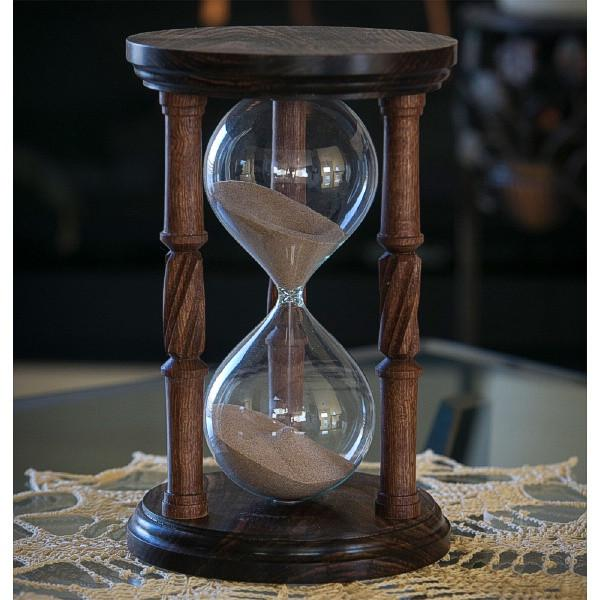
\includegraphics[width=0.4\textwidth]{figs/hourglass_whole.jpg}
    \caption{Two disks in contact with relevant properties labeled for DEM.}
    \label{DEM_diagram}
\end{figure}

In the current work, the contact force, $\bold{f_c}$, is a linear combination of a normal contact force $\bold{f_n}$ and tangential contact force $\bold{f_t}$, such that simply $\bold{f_c} = \bold{f_n} + \mu\bold{f_t}$, where $\mu$ is the coefficient of friction. $\bold{f_d}$ more concretely is
$$\bold{f_n}=k_nd\bold{n}-\gamma_n\bold{v_n}$$
where $k_n$ is the Hookean spring constant in the normal direction, $d$ is the penetration depth between the two disks, $\bold{n}$ is the contact normal unit vector, $\gamma_n$ is the normal damping coefficient, and $\bold{v_n}$ is the normal component of the relative velocity between the two disks. Similarly, the tangential contact force is given by
$$\bold{f_nt}=k_t\Delta\bold{s}-\gamma_t\bold{v_t}$$
where $k_t$ is the spring constant in the tangential direction, $\gamma_t$ is the tangential damping coefficient, and $\bold{v_t}$ is the tangential component of the relative velocity. Friction is captured in this model by requiring that
$$\bold{f_t}\leq\mu\bold{f_n}$$
which is accomplished by adjusting $\Delta\bold{s}$. For a given enduring contact over time, $\Delta\bold{s}$ for that contact is the time integral of the tangential relative velocity during that contact. $\Delta\bold{s}$ is then rescaled so that it $\bold{f_t}$ falls within the friction cone determined by $\mu\bold{f_n}$.

With the given spring-dashpot system, a coefficient of restitution (COR) $e$ can be tuned as a function of the model parameters. Given a desired $e$ and a normal spring coefficient $k_n$, $\gamma_n$ is determined as
$$\gamma_n=\sqrt{mk_n}(-2\log{e})/\sqrt{2(\pi^2+\log{e}^2}$$
where $m$ is the mean mass of a grain \cite{Kamrin:2014}. Note that the use of a "mean" mass is due to the fact that in all of the simulations conducted in this study, a slight polydispersity in granular radii is used with a single density for all particles, resulting in a mass distribution. This is done to better match real shape distributions in a granular system, and to avoid crystallization that commonly arises in monodisperse systems. The choice of $k_n$ and other material parameters is further explained for specific simulations later in the study, but in general is chosen to be as stiff as possible while still retaining a reasonable cost per time step, with a timestep usually on the order of $10^{-6}$ seconds.

\subsection{DEM Algorithm}
The DEM code used in this study was built completely in house, though is similar in general algorithmic structure to many DEM codes that exist, such as LAMMPS or LIGHTS \textcolor{red}{FINDREFERENCE}. Thus for transparency as well as necessity when later explaining the hybrid algorithm, the structure of the used DEM code is discussed.

\begin{algorithm}
  \caption{${\tt Overall \_ DEM \_ Algorithm}$}
  \begin{algorithmic}[1]
  \State ${\tt Broad\_Phase\_Collision\_Detection}$
  \For{$i=0 \dots num\_possible\_collisions$}
    \State ${\tt Narrow\_Phase\_Collision\_Detection}$
  \EndFor
  \State ${\tt Collision\_Update}$
  \For{$each\_collision\_type$}
    \State ${\tt Update\_Properties}$
    \State ${\tt Integrate\_\Delta\bold{s}}$
  \EndFor
  \State ${\tt Force\_Update}$ 
  \For{$each\_collision$}
    \State ${\tt Calculate\_Penalty\_Force}$
    \State ${\tt Correct\_\Delta\bold{s}}$
    \State ${\tt Add\_Force\_To\_Contact\_Grains}$
  \EndFor
  \State ${\tt Time\_Integration}$ 
  \end{algorithmic}
  \label{alg:DEM_algorithm}
\end{algorithm}

The $Broad\_Phase\_Collision\_Detection$ creates an axis-aligned bounding box (AABB) around each grain, and checks the intersection of those AABBs with a background grid. Each grid cell then has a vector of AABBs that intersect it, with each combination of AABB in that vector constituting a possible collision. All possible collisions are then looped over for an actual collision detection ($Narrow\_Phase\_Collision\_Detection$) and any real collisions are added to a vector of actual collisions for a given type. Collision types include, for example, circle\_circle collisions for grains in contact, or circle\_plane collisions for grains in contact with a rigid plane. The list of all collisions for every collision type are then looped over, and properties such as penetration depth and $\Delta\bold{s}$ are updated. With this information, a penalty force is calculated at every contact according to the model presented in \ref{DEM_Model}. With these forces, an explict Forward Euler update is used to numerically integrate the velocity of the grains, which is then used to integrate the position of the grains.

Though dry, cohesionless grains are the focus of the current work, it is noted that the DEM framework allows for a simple extension for cohesive grains. A new collison type can be defined that allows for tracking of grain interactions at a distance. As will be explained later, some initial work has in fact been done on this, by tracking liquid bridges that provide a source of cohesion in the system, in order to extend the hybrid method for cohesive systems.

As a final note, the DEM code is an extension and modification of the SCISIM code developed by Smith for contact dynamics \textcolor{red}{FINDREFERENCE}. In fact, as will be later discussed, that contact dynamics code was first used as the discrete method of choice for the hybrid project. However, the explicit penalty method was determined to better suit the needs of hybridization.
%% This is an example first chapter.  You should put chapter/appendix that you
%% write into a separate file, and add a line \include{yourfilename} to
%% main.tex, where `yourfilename.tex' is the name of the chapter/appendix file.
%% You can process specific files by typing their names in at the 
%% \files=
%% prompt when you run the file main.tex through LaTeX.
\chapter{Continuum Model}

\section{Hyperleastic-Plastic Model}

\section{Hypoelastic-Plastic Model}
In general, hypoelastic models differ from hyperelastic models in that the stress is not obtained from a gradient of a strain energy density function with respect to deformation. The specific hypoelastic granular continuum model used in this study was developed by Dunatunga and Kamrin \cite{Dunatunga:2015:Continuum}. To start one again begins with momentum balance and mass balance
$$\rho\frac{D\bold{v}}{Dt} = \nabla\cdot\bm{\sigma} + \rho\bold{b}$$
$$\frac{D\rho}{Dt} + \rho\nabla\cdot\bold{v}=0$$
with all terms similarly defined as in the hyperelastic model. A useful quantity, the spatial velocity gradient $\bold{L}$, is defined as
$$\bold{L}=\nabla\bold{v}$$
$\bold{L}$ can be decomposed into a symmetric part (known as the strain rate tensor) and skew part (known as the spin tensor), $\bold{D}$ and $\bold{W}$ respectively, such that
$$\bold{L}=\bold{D}+\bold{W}$$
$$\bold{D}=\frac{1}{2}(\bold{L}-\bold{L}^T)$$
$$\bold{W}=\frac{1}{2}(\bold{L}+\bold{L}^T)$$
In contrast to the hyperelastic model, the used hypoelastic model takes an additive split of the strain and strain rate-like terms into an elastic and plastic part. For example,
$$\bold{L}=\bold{L}^e+\bold{L}^p$$
The elastic and plastic spatial velocity gradients can then be decomposed into spin and strain rate tensors
$$\bold{L}^e=\bold{D}^e+\bold{W}^e$$
$$\bold{L}^p=\bold{D}^p+\bold{W}^p$$
A commonly taken assumption that is also taken here is one of spin-less plastic flow, so that $\bold{W}^p=\bold{0}$ and $\bold{L}^p=\bold{D}^p$. Plastic flow codirectionality with the stress deviator and isochoric plastic flow are also taken as assumptions, leading to an plastic flow rate of
$$\bold{L}^p=\bold{\hat{D}}^p(\bm{\sigma})=\frac{1}{\sqrt{2}}\dot{\bar{\gamma}}^p(\bm{\sigma})\frac{\bm{\sigma}_0}{||\bm{\sigma}_0||}$$
where $\dot{\bar{\gamma}}^p$ is the equivalent plastic shear strain rate.

Due to the fact that a hypoelastic-plastic  model is used and there is no tracking of the deformation gradient, an objective rate must be used to update the stress. While many exist, the Jaumann rate is used here as suggested by Dunatunga and Kamrin, and is defined as
$$\stackrel{\triangle}{\bm{\sigma}}=\dot{\bm{\sigma}}-\bm{W}\cdot\bm{\sigma}+\bm{\sigma}\cdot\bm{W}$$


\subsection{Material Point Method}
%% This is an example first chapter.  You should put chapter/appendix that you
%% write into a separate file, and add a line \include{yourfilename} to
%% main.tex, where `yourfilename.tex' is the name of the chapter/appendix file.
%% You can process specific files by typing their names in at the 
%% \files=
%% prompt when you run the file main.tex through LaTeX.
\newcommand{\pluseq}{\mathrel{{+}{=}}}
\chapter{Hybridization}
The previous two chapters described two very different modeling paradigms, both with their strengths and weaknesses. As mentioned in the introduction, the goal is to be able to utilize the strengths of both to offset their weaknesses in order to create a versatile method that can handle phenomena that span many magnitudes of length scales and all phases of granular matter. Namely, the goal is to utilize the accuracy of the discrete element method where it is needed, while in all other regions, using the continuum method to solve a simple continuum model with much fewer degrees of freedom than a full discrete simulation. The method to achieve this is subsequently explained.

\section{Hybridization Overview}
\begin{figure}[htp] 
    \centering
    \includegraphics[width=0.8\textwidth]{figs/hybrid_example.pdf}
    \caption{Diagram of a hybrid simulation.}
    \label{hybrid_diagram}
\end{figure}

Figure \ref{hybrid_diagram} gives a visual representation of a hybrid simulation of a collapsing pile of grains. On the exterior are discrete grains, modeled by DEM. On the interior is a region of continuum, utilizing MPM. A regime where both DEM and continuum overlap each other, what is deemed the "Reconciliation Zone" or "Hybrid Zone" (both are used interchangeably), then connects the two modeling regimes.

From this schematic there are a couple of things of note. A single MPM simulation is used to solve for the pure continuum region, as well as the continuum portion of the hybrid zone. The continuum region has only a single piece of information that delineates the pure continuum from the hybrid continuum: a weight field $w_c(x)$ that has a value of 1 in the pure continuum and a value between 0 and 1 in the hybrid regime. Likewise, a single DEM simulation is used to advance the state of the discrete grains in the pure discrete region as well as the discrete portion of the hybrid zone. Again, a weight field $w_d(x)$ delineates the pure discrete and hybrid regimes, with a value of 1 in the pure discrete region and a value between 0 and 1 in the hybrid region.

At a very high level the hybrid scheme can be described thusly. At the beginning of a hybrid timestep, the domain is decomposed into pure continuum, pure discrete, and hybrid regions. The determination of which region is represented with which model is conducted by what is termed the "oracle", which will be later explained. If the oracle determines that a region described by the continuum model needs greater accuracy, then a process called "enrichment" converts the continuum representation to a discrete representation. On the other hand, if the oracle determines that a discrete region no longer needs to be resolved to that level, then a process called "homogenization" converts that discrete representation into a continuum representation. A step of MPM for what regions are now continuum and a step of DEM for regions that are now discrete are then taken, with no communication between the two regimes other than the weightage split previously described, resulting in intermediary quantities of state. These steps will be referred to as "unconstrained" steps, as they are unconstrained of any coupling between the two distinct systems. A coupling step then acts to kinematically constrain the two partitioned systems in the hybrid zones. These updated quantities are communicated back to the DEM and MPM solvers, which results in the end of timestep quantities for the entire simulation.

The hybrid scheme can be split into three main components. The first is the nature of the split of the continuum and discrete representations in the hybrid zone. The second is the coupling of those two split regions such that they end the step kinematically constrained. The third is the domain decomposition, and the processes of homogenization and enrichment. 

\section{Reconciliation Zone Splitting}
\begin{figure}[htp] 
    \centering
    \includegraphics[width=0.8\textwidth]{figs/blurred_mass.pdf}
    \caption{Blurred Density: (Left) The reference domain $\Omega$ of an object with density $\rho(\bm{x})$. Mass density is colored in blue. (Right) A partition of unity of the density mediated by a weight function $w(\bm{x},t)$.}
    \label{blurred_mass}
\end{figure}

In order to understand the split of the system in the hybrid zone, we introduce a more general system. We start with a body defined over some domain $\Omega$, with a density field $\rho(\bm{x})$. In the hybrid scheme, the domain is decomposed into two different domains according to a weight function that is defined over time and space, $w(\bm{x},t)$ with a range between 0 and 1. The weight function $w$ allows us to decompose any field defined on the body into a linear combination of two separate fields. Taking the density as an example:
\begin{equation}
\rho(\bm{x})=w(\bm{x},t)\rho(\bm{x}) + (1-w(\bm{x},t))\rho(\bm{x})
\end{equation}
To further separate and define the subsystems, let $\bm{q}_1$ and $\bm{v}_1$ define the position and velocity respectively of the first system and $\bm{q}_2$ and $\bm{v}_2$ be the counterparts for the second system. If we impose the constraint that $\bm{q}_1=\bm{q}_2$, then, along with the weight field, we can recover the original system. If we further impose that the initial conditions of both systems are identical, such that $\bm{q}_1(t=0)=\bm{q}_2(t=0)$, then we can define the velocity constraint $\bm{c}(\bm{x},t)=\bm{v}_1(\bm{x},t)-\bm{v}_2(\bm{x},t)=0$.

In order to derive the equations of motion for this decomposed system subject to the velocity constraint $\bm{c}(bm{x},t)$, we formulate the problem in the context of Lagrangian mechanics, using Hamilton's Variational Principle \cite{Lanczos:2012}. From this point one, the time and space dependence on the quantities of interest are excluded for brevity. We introduce the kinetic energy $T$ and potential energy $U$ of the decomposed system, defined as
\begin{align}
\begin{aligned}
T &= \frac{1}{2} \int_\Omega \rho w \bm{v}_1^T \bm{v}_1 dV + \frac{1}{2} \int_\Omega \rho (1-w) \bm{v}_2^T \bm{v}_2 dV, \\
U &= \int_\Omega \rho w e[\bm{q}_1] dV + \int_\Omega \rho (1-w) e[\bm{q}_2] dV,
\end{aligned}
\end{align}
for potential energy per unit mass $e$. We then introduce the constraint $C$ defined by
\begin{equation}
C = \int_\Omega \bm{\lambda}^T (\bm{v}_1 - \bm{v}_2) \,dV
\end{equation}
where $\lambda\left(\mathbf{x},t\right)$ is a
Lagrange multiplier field. With the Lagrangian $L=T-U+C$, we apply the calculus of variations to obtain the Euler-Lagrange equations for the decomposed system:
\begin{align}
\label{eq:coupling}
%\left\{
\begin{aligned}
\int_\Omega w \rho \bm{a}_1 \,dV = - \int_\Omega w \underbrace{\rho \frac{\delta e}{\delta \bm{q}_1}}_{\frac{\text{Force}}{\text{Volume}}_1} \,dV - \underbrace{\int_\Omega \bm{\lambda}\, dV}_{\textrm{\scriptsize  coupling force}} , \\
\int_\Omega (1-w) \rho \bm{a}_2 \,dV = - \int_\Omega (1-w) \underbrace{\rho \frac{\delta e}{\delta \bm{q}_2}}_{\frac{\text{Force}}{\text{Volume}}_2} \,dV + \underbrace{\int_\Omega \bm{\lambda}\, dV}_{\footnotesize\textrm{\scriptsize  coupling force}} ,
\end{aligned}
%\right.
\end{align}
under the kinematic constraint that $\bm{v}_1=\bm{v}_2$. The Lagrange multiplier can conveniently be interpreted as a coupling force that acts equally and oppositely on both systems, in order to obtain a matching velocity field in both systems. Summing the equations for the two systems recovers the original system, displaying a partition of unity for the decomposition. 

We now replace these two abstract systems with a discrete particle system and a continuum system. We require the stress in the continuum domain to be compatible with the homogenized frictional forces in the discrete domain. This homogenization is realizable through the so-called Christoffersen formula \cite{Christoffersen:1981:Micromechanical}, which relates the continuum stress to the discrete frictional contact forces via:
\begin{align}
\sigma_{ij} = \frac{1}{V} \sum_{\alpha \in contacts}^{N}{\frac{1}{2}(\boldsymbol{f}_i^\alpha \boldsymbol{d}_j^\alpha + \boldsymbol{f}_j^\alpha \boldsymbol{d}_i^\alpha)} , 
\end{align}
where $\sigma_{ij}$ is the (i,j) component of the stress tensor, $V$ is the volume 
about which one is homogenizing the stress, $N$ is the number of contacts in 
that volume, $\boldsymbol{f}_i^\alpha$ is the $i^{th}$ component of the contact 
force vector at the $\alpha^{th}$ contact, and $\boldsymbol{d}_i^\alpha$ is the
$i^{th}$ component of the vector connecting the centroids of the two grains in contact.

\section{Coupling Constraints}
With the integrated equations of motion derived from the Euler-Lagrange equations, we can derive the position and velocity updates for the separate continuum and discrete systems in the hybrid zone, where the Lagrange multiplier acts to correct the two system updates to kinematically agree with each other. The continuum nature of the continuum portion of the simulation allows us to define a velocity field everywhere in the pure continuum and hybrid portions of the domain. The kinematic constraint therefore enforces that at every discrete particle location, the discrete particle velocity is identical to the interpolated continuum velocity field at that location, enforcing the constraint in an averaged continuum sense \cite{Bergou:2007:TTDTS}. Letting the reconciliation zone be defined on a domain $\Omega_R$, and letting $\lambda_k$ represent the constraint force on the $k$th discrete particle, the $p$th
material point moves as
\begin{align}
\begin{aligned}
&\frac{d}{dt} \boldsymbol{q}_p = \bm{v}_p , \\
&\frac{d}{dt} (w_p M_p \bm{v}_p) = \underbrace{\frac{d}{dt} (w_p M_p \bm{v}_p^*) \sum_{k \in \Omega_R} }_{\textrm{\scriptsize unconstrained step}} \hspace{6pt} \underbrace{- \sum_{k \in \Omega_R} \Gamma_{pk}\lambda_k}_{\textrm{\scriptsize constrained step}} ,
\end{aligned}
\end{align}
while the $k$th discrete particle moves as
\begin{align}
\begin{aligned}
&\frac{d}{dt} \boldsymbol{q}_k = \bm{v}_k , \\
&\frac{d}{dt} ((1-w_k) M_k \bm{v}_k) = \underbrace{\frac{d}{dt} ((1-w_k) M_k \bm{v}_k^*)}_{\textrm{\scriptsize unconstrained step}} \underbrace{\hspace{20pt} + \boldsymbol{\lambda}_k  \hspace{20pt} {\frac{d}{dt}}}_{\textrm{\scriptsize constrained step}} ,
\end{aligned}
\end{align}
where $\bm{v}_p^*$ and $v_k^*$ are the predictions from continuum and discrete simulations respectively before coupling forces are added, and
$\Gamma_{pk}$ are material-point to discrete-particle interpolation coefficients, defined by the same basis functions used in the pure continuum region to interpolate the point properties to the grid.

\subsection{Hybrid Coupling Discretization} \label{subsec:hybrid_coupling_discretization}
The hybrid coupling algorithm in the context of the complete simulation routine is now discussed. In order to integrate in time, we choose an explicit scheme for all components: the discrete method, the continuum method, and the hybrid coupling. While the usual stability tradeoff is made in using an explicit scheme over an implicit scheme, we note that the simplification in the system of equations that results is, for now, worth the computational cost. The scheme can therefore be interpreted as a predictor-corrector scheme, where the DEM and MPM algorithms produce predictor quantities, and the hybrid coupling produces a corrector, applied at the end of the step. As an aside we also note that having consistent schemes across all simulations is important for coupling accuracy. Previous attempts were made to couple a contact dynamics method to the explicit MPM method used to advance the continuum. Because contact dynamics is implicit, the scheme produces a result that is consistent with the constraints defined only in the pure discrete system. Applying a corrector step to the the resulting quantities essentially throws away these constraint. Contact dynamics also assumes completely rigid particles, which does not match the finite elasticity of the constitutive law used for the continuum. The macroscopic phenomenological effects of these discrepancies was that discrete particles slowly drifted through static hybrid zones.

Thus using the explicit schemes previously described, the hybrid coupling occurs as follows. First, an unconstrained step is taken by the discrete method, producing discrete predictor momentum $M_dv^*_d$ and forces $f^*_d$. The predictor position is discarded. An unconstrained MPM step is then taken up to and including the updateNodalMomentum step of Algorithm \ref{alg:MPM_algorithm}, resulting  resulting in continuum predictor momentum $M_cv^*_c$ and forces $f^*_c$ defined on the grid. The hybrid weight field in the hybrid zone $w$ is incorporated into the DEM by multiplying the spring constants $k_n$ and $k_t$ by $1-w$ and the mass of each particle by $1-w$, when solving for the forces on each grain at the $Force\_Update$ step of Algorithm \ref{alg:DEM_algorithm}. In the continuum, the stress and mass are weighted by $w$, which appear any time the mass or stresses are projected to and from the grid. The predictor quantities form the RHS of a system of equations for the corrected coupled system, which in matrix form is defined as:
\begin{align}
\begin{bmatrix}
    W_c M_c & 0 & \Gamma_c \\
    0 & W_d M_d & -\Gamma_d \\
    \Gamma_c^T & -\Gamma_d^T & 0
\end{bmatrix}
\begin{bmatrix}
    \bm{v}_c^{n+1} \\
    \bm{v}_d^{n+1} \\
    \lambda
\end{bmatrix}
=
\begin{bmatrix}
    W_c \left( M_c \bm{v}^*_c + h \bm{f}^*_c \right) \\
    W_d \left( M_d \bm{v}^*_d + h \bm{f}^*_d \right) \\
    0
\end{bmatrix}
\label{eq:coupled_system}
\end{align}
where $W_c$ and $W_d$ are diagonal matrices that contain the mass weights for the continuum and discrete systems and $\bm{\lambda}$ are the Lagrange multipliers. Solving the linear system gives the corrected continuum and discrete velocities $\bm{v}_c^{n+1}$ and $\bm{v}_d^{n+1}$.
$\Gamma_d$ and $\Gamma_c$ are defined such that
$\Gamma_d^T \bm{v}_d - \Gamma_c^T \bm{v}_c$ produces the residual relative velocity of discrete bodies within the background
velocity field defined by the material point grid. Thus $\Gamma_d$ is the identity matrix,
while each column of $\Gamma_c$ contains the combination of weights, obtained from the MPM basis functions, that reconstruct a DEM grain's mass. We use as arguments for the basis functions $\bm{x}^n_p$ and $\bm{x}^n_d$, the positions of the material points and discrete bodies respectively at the beginning of the unconstratined steps.

With the corrected constrained velocities for both systems, we communicate this information back to the DEM and MPM algorithm. The discrete grains are advected according to the corrected velocity $v^{n+1}_d$, completing a discrete timestep. In the MPM simulation, we overwrite the * momentuma on the nodes obtained after the updateNodalMomentum step, and proceed with the rest of the MPM algorithm. With these separate systems evolved, the hybrid step is complete.

\subsection{Nodal Coupling}
When implemented, the coupling method presented works, and was used as a proof of concept on a number of toy problems. However, a linear system solve is usually a bottleneck in numerical methods, and this proved to be true here as well. Despite the fact that the linear solve is only on the relatively small hybrid portion of a simulation domain, the coupling matrix still proved to be large in absolute terms. The usual suite of solutions were tried, such as using iterative solvers and parallelizing the matrix solve, but ultimately the hybrid system solve time was constrained by this large matrix.

To address this issue and greatly simplify the system, we move to coupling the discrete system in an element-averaged sense, similar to the continuum system. In essence, we treat the discrete grains like material points, and apply the projection operator defined by (\ref{projection_value}) to get nodal representations of the discrete mass and momentum on a grid that is colocated to the MPM grid. In the context of \ref{eq:coupled_system}, $\bm{\Gamma}_c$ and $\bm{\Gamma}_d$ both reduce to identity. We then constrain these nodal discrete and nodal continuum momenta. What results is a system of equations on each hybrid node:
\begin{align}
W_c M_c \bm{v}_c^{n+1} + \lambda &= W_c M_c \bm{v}^*_c , \label{eq:sys_a} \\
W_d M_d \bm{v}_d^{n+1} - \lambda &= W_d M_d \bm{v}^*_d , \label{eq:sys_b} \\
\bm{v}_c^{n+1} &= \bm{v}_d^{n+1} . \label{eq:sys_c}
\end{align}
Substituting $\bm{v}_c^{n+1}$ for $\bm{v}_d^{n+1}$ in Eq. \eqref{eq:sys_a}, adding Eq. \eqref{eq:sys_a} and Eq. \eqref{eq:sys_b},
and solving for $\bm{v}_d^{n+1}$, we find that:
\begin{align}
\label{eq:inexpensive_coupling}
\bm{v}_c^{n+1} = \bm{v}_d^{n+1} = \left( W_c M_c + W_d M_d \right)^{-1} \left( W_c M_c \bm{v}_c^* + W_d M_d \bm{v}_d^* \right) .
\end{align}
The constrained velocities can now be interpreted as an
inelastic impact between two particles in one dimension at each hybrid grid node. An important quality of this approach is that the hybrid nodes uncouple, with the solution at each grid node being independent of the other grid nodes. Because only a single equation is being solved at each coupled node, this coupling method is very quick, and can also be trivially parallelized. We also avoid numerical issues such as having to solve an ill-conditioned matrix.

These new corrector momenta are treated in the same way as before in the MPM system, overwriting the * momenta values and the MPM algorithm is advanced as usual. For the discrete representation, the corrector nodal quantities are projected back to the discrete grains in the exact same way as the MPM, described in the updatePointVelocities step. This though carries with it the choice of a PIC or FLIP update, and we choose the $\alpha$ parameter to be the same as that for the MPM method. In practice, we always use this grid version of the coupling scheme because of its numerous advantages.

\section{Domain Decomposition}

\subsection{Oracle}

\begin{figure}[htp] 
    \centering
    \includegraphics[width=0.8\textwidth]{figs/hybrid_zone_update.pdf}
    \caption{Initialization of a hybrid simulation: (A) We begin with a collection of DEM grains. (B) We next locate a level
    set corresponding to a given low density, here denoted as a black line. (C) Across the domain, we compute
    the distance to the density threshold, indicated by lines in lighter shades of red as the distance increases.
    (D) We select a user-tunable distance to the density level-set that serves as the center of the hybrid
    ``reconciliation" zone. We denote this critical distance as a solid black line. (E) We extend the hybrid zone
    along the distance field by a given half-width in each direction, indicated by dotted lines. This hybrid
    reconciliation zone between the dotted lines defines a zone where the DEM system will be coupled to the
    continuum system. We homogenize the velocity and stress for use in step (G). (F) We delete all discrete grains that fall within the inner boundary of the reconciliation zone.
    (G) We run the "avoid-a-void" algorithm of Yue et al. \cite{Yue:2015:Continuum} from the outer boundary in to populate the region with material points. The material point states are determined using the homogenized velocity and stress computed in step (E).}
    \label{hybrid_initialization}
\end{figure}
Now that we have defined the coupling in the hybrid zone, we have fully defined the equations of motion in all regions of the domain and can integrate those regions in time and space. The next component of the hybrid algorithm then is determining how the entire domain is decomposed into those different regions. The mechanism that does this is deemed the "oracle"; given the current state of the simulation, the oracle tells us what regions are safe to be modeled via continuum and which regions need the higher resolution discrete model. The oracle itself opens up a deeper field of inquiry, as it essentially asks what properties in a granular flow are most important in capturing the different behaviors of that flow. 

As a first pass, we consider a number of scenarios where simple continuum laws cannot accurately capture behaviors of interest. Grain-scale level behaviors, such as breaking off of individual grains from a pile, cannot be well captured by a continuum model. Geometries and flows where finite-size effects in general are important are difficult to capture, such as the jamming of a silo due to arch formation near the silo orifice \cite{Beverloo:1961:Flow,Midi:2004:Dense,Pouliquen:1999:Scaling,Sheldon:2010:Granular}. Areas with high-strain rates, resulting in very non-affine motion, are also difficult to capture in continuum \cite{Dijksman:2010:Granular,Kamrin:2010,Koval:2009:Annular}. Free surface flows, and the interaction of multiple granular bodies at their respective free surfaces, are also difficult to model with continuum models, with the possible need to define contact models.

A convenient proxy that tends to delineate when these processes are or are not occurring is the granular packing fraction. For example, at the free surface of a granular body, the packing fraction goes to 0. Breakaway particles also have a low packing fraction, where a representative volume will only capture a few grains. Our current oracle therefore takes as its input measurements of the packing fraction.

At the beginning of a hybrid update, the packing fraction of the pure discrete system is calculated via the use of a background grid. We take the grid divisions to be an integer multiple of the MPM and hybrid grids. Any elements in the packing fraction grid that are co-located with a hybrid or MPM zone defined on the hybrid grid are marked as having a packing fraction of 1. The elements corresponding to pure discrete zones are calculated via area or volume intersections of the grains with the grid element they are in. From this $\Phi$ field  we can construct an packing field isocontour corresponding to a user-adjustable critical packing, $\Phi_c$. $\phi_0$, another user-adjustable parameter, is the distance away from the $\Phi$ contour deemed safe for the continuum model. Finally, the reconciliation zone half-width, $r_h$, is used in conjunction with the other parameters to establish the zone types. Elements are hybrid if the distance of that element to the isocountour $\Phi_c$ is  
$\phi_0 - r_h \leq \Phi_d(\bm{x}) \leq \phi_0 + r_h$. Zones are marked continuum if $\Phi_d(\bm{x}) > \phi_0 - r_h$ and discrete if $\Phi_d(\bm{x}) < \phi_0 + r_h$.

\subsection{Homogenization and Enrichment}
\label{sec:enrichment}
With the domain decomposition machinery defined, the final step in fully defining the hybrid scheme is to determine how to convert between the various representations. It should be noted that we do not allow conversions from pure discrete regions to pure continuum regions and vice versa, forcing them to transition through a hybrid regime. This results in a smoother transition in time between the two representations and also ensures that there is always a hybrid zone between pure discrete and pure continuum elements. If a simulation starts with only discrete grains, then we run the following scheme twice, first transitioning the interior to a hybrid representation, then again, converting the interior hybrid zones to continuum.

We therefore must account for four different types of zone conversions: hybrid to discrete, hybrid to continuum, discrete to hybrid, and continuum to hybrid. For the hybrid to discrete conversion, any material points in the element are deleted and the discrete grains are kept unmodified (other than their weight function $w$). Similarly, in the hybrid to continuum conversion, any discrete grains are deleted and the continuum weights are changed but are otherwise left alone. The conversions to hybrid zones are a little more involved, as creation is more difficult than deletion. In going from discrete to hybrid, material points must be introduced in manner such that the now weighted discrete grains and new weighted material points sum to be consistent with the pure discrete system. The must occur for new grains in converting from continuum to hybrid zones. In order to introduce new points and grains to new hybrid zones, we utilize the "Avoid a Void" (AA) sampling algorithm developed by Yue et al in the context of improved MPM point sampling \cite{Yue:2015:Continuum}. AA utilizes Poisson-disk sampling to generate the location of new points in a random but spatially uniform manner, helping to ensure that the position of the MPM points (which are also the continuum quadrature points) are visually well distributed but also result in satisfactory integration.

Therefore, to convert from discrete to hybrid zones, new MPM points are injected at locations determined from AA. To initialize the properties of the points, we homogenize the discrete grain properties. A new background grid is introduced, co-located with the hybrid grid. We utilize the MPM basis functions to project the mass and momentum of the discrete grains to the nodes of this grid, and obtain nodal velocities from those quantities. We then use the basis functions again to interpolate this grid velocity at the location of the new MPM points, and assign those velocities to those points. We also homogenize the stress of the discrete grains with the Christoffersen formula, and project those stresses to the nodes. Again we interpolate this field to get the MPM point stresses. We then determine the strain field by utilizing the constitutive law. For the hyperelastic model, we obtain $\bar{\bm{B}}^e$ by utilizing the fact that $dev[\bar{\boldsymbol{B}}^e] = \frac{J}{\mu} dev[\bm{\sigma}]$ and $\bar{\boldsymbol{B}}^e = dev[\bar{\boldsymbol{B}}^e] + t \boldsymbol{I}$,
and we solve for $t$ with $det[\bar{\boldsymbol{b}}^e] = 1$. 
%We emphasize the importance of syncing the stress and strain during homogenization to
%preserve volume. Previously, we initialized new continuum elements to a stress-free state.
%This stress-free initialization caused the material to gain volume if the discrete grains were between a gaseous and liquid state while separating, however.

To introduce discrete grains, we introduce grains with a radius determined from a given distribution, and again pick new locations according to the AA algorithm. Here, there is the additional constraint that new grains must not overlap other grains. It should be noted that this is not entirely symmetric with the homogenization process; in homogenization we determine a continuum stress field from a discrete force network but in enrichment we do not establish a force network from a continuum stress field. This is because the latter is an ill-posed problem, and would require a possible optimization process to determine. We note that this is a future area of work, and justify the current lack of force network formation by the observation that in practice, the discrete grains quickly form appropriate contact networks in the hybrid zone and these transients do not seem to affect the overall dynamics of the problem at a noticeable level. The initial velocity of new discrete grains is computed by averaging the velocity of surrounding discrete grains and material points within a radius of $6$ (mean) grain diameters, with an exponential
falloff. This window width is slightly above the minimal size that recovers
continuum-like quantities in a "granular volume element" \cite{Rycroft:2009}.

\subsection{Optimized Zone Decomposition}
\label{sec:layered_3D}
The 3D generalization of Figure \ref{hybrid_initialization} can be visualized as a spheroid of discrete grains, with the interior volume replaced by continuum. Visually, one only sees the exterior grains. However in practice, one does not need even this many grains visible or needed as free surface. Take for example sand in a sandbox. The oracle in that situation would take away the material in the middle of the box, but leave the grains on the free surface and all sides touching the box. What is only really needed is the grains at the free surface, for any possible objects that fall into or interact with the sand. We therefore introduce a \textit{layered hybridization}, where only a single surface is discrete grains, and the rest of the surfaces and interior are all continuum. This results in a further reduction in the discrete grain count, pushing possible speedup gains higher. We apply this approach to the bunny toss, excavator, bunny drill, and tire examples in Chapter~\ref{sec:results}.
%
%\begin{algorithm}
%\caption{${\tt Identify \_ Hybrid \_ Zones}$}
%\begin{algorithmic}[1]
%\State $\Phi_{\rho} \gets {\tt Discrete \_ Packing \_ Fraction \_ Isocontours}\left(\boldsymbol{q}_d\right)$
%\State $\Phi_{d} \gets {\tt Distance \_ to \_ Density \_ Isocontours}\left(\Phi_{\rho}\right)$
%\State ${\tt continuum \_ zone}\left( \mathbf{x} \right) \gets \Phi_{d}\left( \mathbf{x} \right) > \phi_0 - r_h$
%\State ${\tt discrete \_ zone}\left( \mathbf{x} \right) \gets \Phi_{d}\left( \mathbf{x} \right) < \phi_0 + r_h$
%\State ${\tt hybrid \_ zone}\left( \mathbf{x} \right) \gets \phi_0 - r_h \leq \Phi_{d}\left( \mathbf{x} \right) \leq \phi_0 + r_h$
%\end{algorithmic} \label{alg:identify_hybrid_zones}
%\end{algorithm}
%
%\begin{algorithm}
%\caption{${\tt Update \_ Hybrid \_ Zones}$}
%\begin{algorithmic}[1]
%\State ${\tt Homogenize \_ Velocity \_ and \_ Stress}\left( {\tt hybrid \_ zone} \right)$ 
%\State ${\tt Discrete \_ Avoid \_ a \_ Void}\left( {\tt hybrid \_ zone} \right)$ 
%\State ${\tt Continuum \_ Avoid \_ a \_ Void}\left( {\tt hybrid \_ zone} \right)$ 
%\State ${\tt Delete \_ Discrete \_ Grains}\left( {\tt continuum \_ zone} \right)$ 
%\State ${\tt Delete \_ Continuum \_ Particles}\left( {\tt discrete \_ zone} \right)$ 
%\end{algorithmic} \label{alg:update_hybrid_zones}
%\end{algorithm}
%
%\begin{algorithm}
%\caption{${\tt Update \_ Hybrid \_ State}$}
%\begin{algorithmic}[1]
%\State ${\tt Identify \_ Hybrid \_ Zones}$
%\State ${\tt Update \_ Hybrid \_ Zones}$
%\end{algorithmic} \label{alg:update_hybrid_state}
%\end{algorithm}
%
%\begin{algorithm}
%\caption{${\tt Create \_ Discrete \_ Grain}$}
%\begin{algorithmic}[1]
%\State $\mathbf{x} \gets {\tt Position \_ from \_ Avoid \_ a \_ Void}$
%\State $r \gets N\left( r_{mean}, r_{sigma} \right)$ \Comment{Normally distributed radii}
%\State $m \gets \frac{4}{3} \pi r ^ 3$
%\State $\mathbf{v} \gets 0$
%\State $W \gets 0$
%\For{$i=0 \dots N_d$} \Comment{Iterate over discrete grains}
%  \If{$\left| \mathbf{x}_i - \mathbf{x} \right| < 12 \ r_{mean}$}
%    \State $w \gets e^{ \left| \mathbf{x}_i - \mathbf{x} \right|^2 / 2 r_{mean}^2}$
%    \State $\mathbf{v} \gets \mathbf{v} + w \ \mathbf{v}_i$
%    \State $W \gets W + w$
%  \EndIf
%\EndFor
%\For{$i=0 \dots N_c$} \Comment{Iterate over material points}
%  \If{$\left| \mathbf{x}_i - \mathbf{x} \right| < 12 \ r_{mean}$}
%    \State $w \gets e^{ \left| \mathbf{x}_i - \mathbf{x} \right|^2 / 2 r_{mean}^2}$
%    \State $\mathbf{v} \gets \mathbf{v} + w \ \mathbf{v}_i$
%    \State $W \gets W + w$
%  \EndIf
%\EndFor
%\State $\mathbf{v} \gets \mathbf{v} / W$
%\end{algorithmic} \label{alg:create_discrete_grain}
%\end{algorithm}
%
%\begin{algorithm}
%\caption{${\tt Homogenize \_ Velocity \_ and \_ Stress}$}
%\begin{algorithmic}[1]
%\For{each ${\tt body} \in {\tt Discrete \_ Grains}$}
%  \For{${\tt node} \in {\tt Stencil(body)}$}
%    \State $w \leftarrow {\tt Weight(body, node)}$
%    \State ${\tt node.m } \pluseq w \cdot {\tt body.m }$
%    \State ${\tt node.momentum} \pluseq w \cdot {\tt body.m } \cdot {\tt body.}\bm{v}$
%  \EndFor    
%\EndFor
%\For{${\tt node} \in {\tt Grid \_ Nodes}$}
%  \If{${\tt node.m} > 0$}
%    \State ${\tt homogenized \_ velocity} \leftarrow {\tt node.momentum} /  {\tt node.m}$
%  \EndIf
%\EndFor
%\For{each ${\tt c} \in {\tt collisions}$}
%  \For{${\tt node} \in {\tt Stencil(c)}$}
%    \State $w \leftarrow {\tt Weight(c, node)}$
%    \State $\boldsymbol{f}_c \leftarrow {\tt c}.{\tt collision \_ force}$ \Comment{Normal and friction forces}
%    \State $\boldsymbol{r}_c \leftarrow {\tt c}.{\tt arm \_ vector}$
%    \State $\bm{\sigma}_c \leftarrow \frac{1}{2} \left( \boldsymbol{f}_c  \boldsymbol{r}_c^T + \boldsymbol{r}_c \boldsymbol{f}_c^T \right)$
%    \State ${\tt homogenized \_ stress } \pluseq w \cdot \bm{\sigma} / {\tt cell \_ volume}$
%  \EndFor
%\EndFor
%\end{algorithmic} \label{alg:homogenize_stress}
%\end{algorithm}
%
%\begin{algorithm}
%\caption{${\tt Discrete \_ Avoid \_ a \_ Void}$}
%\begin{algorithmic}[1]
%  \For {${\tt cell} \in {\tt Hybrid \_ Zone}$}
%    \For {$i=0 \dots {\tt Max \_ Iters}$}
%      \State ${\tt Create \_ Discrete \_ Grain}()$
%    \EndFor
%  \EndFor
%\end{algorithmic} \label{alg:discrete_avoid_a_void}
%\end{algorithm}
%
%\begin{algorithm}
%\caption{${\tt Create \_ Continuum \_ Particle]}$}
%\begin{algorithmic}[1]
%\State $\mathbf{x} \gets {\tt Position \_ from \_ Avoid \_ a \_ Void}$
%\end{algorithmic} \label{alg:create_continuum_particle}
%\end{algorithm}
%
%\begin{algorithm}
%\caption{${\tt Reassign \_ Hybrid \_ Continuum \_ Properties}$}
%\begin{algorithmic}[1]
%  \For {${\tt point} \in {\tt Cell}$}
%    \State ${\tt point.m} \leftarrow {\tt mpm \_ mass \_ per \_ cell} / ({\tt \#points} \in {\tt Cell}) $
%    \State ${\tt point.vol} \leftarrow {\tt cell \_ volume} / ({\tt \#points} \in {\tt Cell}) $
%    \State ${\tt point.}\boldsymbol{v} \leftarrow {\tt homogenized \_ velocity} ({\tt point.}\boldsymbol{x}) $
%    \State $\boldsymbol{\sigma} \leftarrow {\tt homogenized \_ stress} ({\tt point.}\boldsymbol{x})$ 
%    \State ${\tt point.strain} \leftarrow {\tt convert \_ stress \_ to \_ strain} (\boldsymbol{\sigma}) $
%  \EndFor
%\end{algorithmic} \label{alg:determine_properties_for_hybrid_continuum_particles}
%\end{algorithm}
%
%\begin{algorithm}
%\caption{${\tt Determine \_ New \_ Inner \_ Continuum \_ Properties}$}
%\begin{algorithmic}[1]
%  \For {${\tt newly \_ sampled \_ point} \in {\tt Cell}$}
%    \State ${\tt point.m} \leftarrow {\tt gather \_ mass \_ of \_ extant \_ nghbr \_ pnts} $
%    \State ${\tt point.vol} \leftarrow {\tt gather \_ vol \_ of \_ extant \_ nghbr \_ pnts} $
%    \State ${\tt point.}\boldsymbol{v} \leftarrow {\tt interp \_ vel \_ of \_ extant \_ nghbr \_ pnts} $
%    \State ${\tt point.strain} \leftarrow {\tt interp \_ strn \_ of \_ extant \_ nghbr \_ pnts} $
%  \EndFor
%\end{algorithmic} \label{alg:determine_properties_for_new_inner_continuum_particles}
%\end{algorithm}
%
%\begin{algorithm}
%\caption{${\tt Continuum \_ Avoid \_ a \_ Void}$}
%\begin{algorithmic}[1]
%  \For {${\tt cell} \in {\tt Hybrid \_ Zone}$}
%    \For {$i=0 \dots {\tt Max \_ Iters}$}
%      \State ${\tt Create \_ Continuum \_ Particle}()$
%    \EndFor
%    \State ${\tt Reassign \_ Hybrid \_ Continuum \_ Properties}$
%  \EndFor
%  \For {${\tt cell} \in {\tt Continuum \_ Zone}$}
%    \For {$i=0 \dots {\tt Max \_ Iters}$}
%      \State ${\tt Create \_ Continuum \_ Particle}()$
%    \EndFor
%    \State ${\tt Determine \_ New \_ Inner \_ Continuum \_ Properties}$ 
%  \EndFor
%\end{algorithmic} \label{alg:continuum_avoid_a_void}
%\end{algorithm}
%
%\begin{algorithm}
%  \caption{${\tt Delete \_ Discrete \_ Grains}$}
%  \begin{algorithmic}[1]
%  \For{${\tt body} \in {\tt Discrete \_ Grains}$}
%    \If{${\tt body} \in {\tt Continuum \_ Zone}$}
%      \State ${\tt delete} \left({\tt body}\right)$  
%    \EndIf
%  \EndFor
%  \end{algorithmic}
%  \label{alg:delete_discrete_grains}
%\end{algorithm}
%
%\begin{algorithm}
%  \caption{${\tt Delete \_ Continuum \_ Particles}$}
%  \begin{algorithmic}[1]
%  \For{${\tt point} \in {\tt Material \_ Points}$}
%    \If{${\tt point} \in {\tt Discrete \_ Zone}$}
%      \State ${\tt delete} \left({\tt point}\right)$  
%    \EndIf
%  \EndFor
%  \end{algorithmic}
%  \label{alg:delete_continuum_particles}
%\end{algorithm}

\chapter{Results} \label{sec:results}
To benchmark the hybrid technique we employ the method on a number of model problems. In all of the following simulations we use a weight of uniform weight of $0.5$ for both the discrete and continuum components in the hybrid zones. Unless otherwise stated, the simulations utilized an MPM cell width to DEM grain diameter ratio of 2:1. We also utilize the hyperelastic formulation to model the continuum regions in all simulations. 

\begin{table}[!htb]
  %\begin{tabular}{|p{1.7cm}|p{0.7cm}|p{1.0cm}|p{0.7cm}|p{0.8cm}|p{1.0cm}|}
  \begin{tabular}{llllll}
      \hline
      \textbf{Simulation} & \textbf{DEM Cost} & \textbf{Hybrid Cost} & \textbf{Total Cost} & \textbf{Speedup} & \textbf{DEM Grains}\\
      \hline
      Silo, DEM    & 0.41 & N/A & 0.41 & N/A  & 100,000\\
      Silo, Hybrid & 0.25 & 0.03 & 0.28 & $1.47\times$ & 78,538\\
      \hline
      Toss, DEM    & 0.620 & N/A & 0.620 & N/A  & 120,000\\
      Toss, Hybrid & 0.164 & 0.193 & 0.357 & $1.74\times$ & 28,289\\
      \hline
      Drill, DEM    & 1.84  & N/A  & 1.84  & N/A & 360,000\\
      Drill, Hybrid & 0.125 & 0.145 & 0.27 & $6.82\times$ & 42,933\\
      \hline
      Tires, DEM    & 3.60 & N/A & 3.60 & N/A  & 588,320\\
      Tires, Hybrid & 0.54 & 0.51 & 1.05 & $3.43\times$ & 114,35\\
      \hline
  \end{tabular}
  \vspace{0.2cm}
  \caption{Simulation performance. Timings of our hybrid approach compared to a purely discrete approach for different scenarios. All reported costs have units of average seconds per time step. The hybrid cost includes both the cost of MPM time evolution and the coupling solves. We take a constant DEM time step of $dt=10^{-6}$ and a constant MPM time step of $dt=10^{-5}$. We gathered all performance statistics on an Intel 3.5 GHz Core i7-4770K with a single thread.} \label{tbl:speedup}
\end{table}

%\input{result_granular_column_collapse.tex}

%\input{result_silo_discharge.tex}

%\input{result_bunny_drill.tex}

%\input{result_drum.tex}

%\input{result_speedup.tex}

%\input{result_core_scaling.tex}

\section{Granular Column Collapse}
In Fig.~\ref{fig:hybrid:column_collapse}, we simulate a collapsing column
with pure DEM and with our hybrid approach. Note the correspondence between the shapes of both
piles. Further observe that our hybrid method captures detailed ``fly away'' effects -- individual grains
separate from the overall bulk and roll away at the front of the collapse, a visually important effect that
would be difficult to capture with a purely continuum model.

\begin{figure}
  \centering
  \includegraphics[width=0.8\linewidth]{figs/column_collapse.pdf}
  %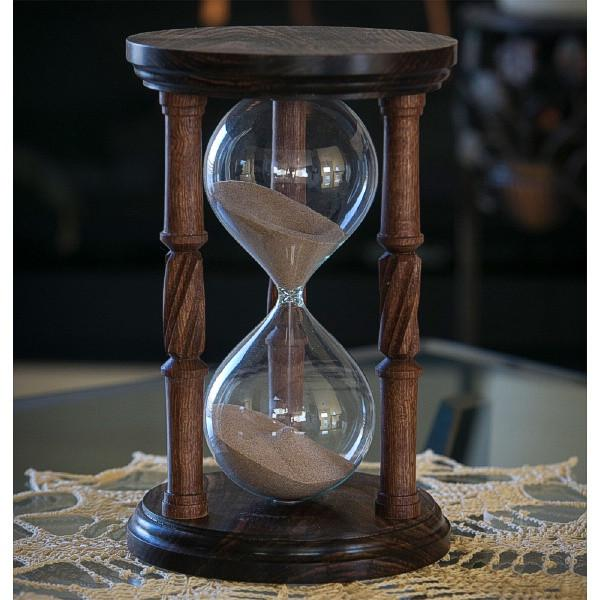
\includegraphics[width=0.4\textwidth]{figs/hourglass_whole.jpg}
  \caption{
    Granular column: A collapsing column simulated with DEM (top) and with our hybrid approach
    (bottom). Observe the nice agreement in the final profile with our hybrid approach and the purely DEM approach.
  }
  \label{fig:hybrid:column_collapse}
\end{figure}

Encouraged by the agreement between the pure DEM approach and our hybrid approach, we validated our hybrid
model against the power-law scaling of the run-out distance $\delta d = d_f - d_i$ reported in the literature,  
where $d_f$ is the distance from the left wall (for a unilateral collapse like our study, or from the column center for a bilateral collapse) to the center of mass of the foremost grain that is connected to the main collection of grains, and $d_i$ is the initial column width (for a unilateral collapse, or the initial half-width for a bilateral one), as in Fig.~\ref{fig:hybrid:column_collapse}.
Granular run-out in a column follows a power law scaling as a function of the initial aspect ratio $AR = h_i / d_i$ in both experimental \cite{Lube:2005,Balmforth:2005}
and numerical \cite{Staron:2005,Lagree:2011,Mast:2015,Dunatunga:2015:Continuum} tests, where $h_i$ is the initial height of the column. Running a series of run-out
simulations over a range of aspect ratios, we corroborate the previously reported power law scaling.
Below a critical aspect ratio, we observe a linear run-out distance as a function of aspect ratio. Above this
threshold, we observe a second power law scaling.

\begin{figure}
  \centering
  \includegraphics[width=0.7\linewidth]{figs/runout_curve.pdf}
  %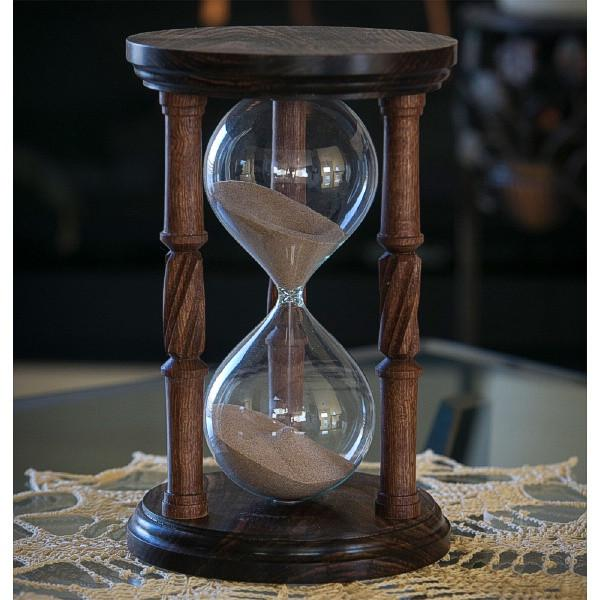
\includegraphics[width=0.4\textwidth]{figs/hourglass_whole.jpg}
  \caption{
    Runout of a 2D granular column: Nondimensionalized runout distance, $\delta d/d_i=(d_f-d_i) / d_i$, vs aspect ratio, $AR = h_i / d_i$. Like DEM, our hybrid technique captures the two distinct regimes that Lube \cite{Lube:2005} observed in experiments. We perform a linear fit in the low-$AR$ regime, and a power-law fit in the high-$AR$ regime.}
  \label{fig:hybrid:runout_curve}
\end{figure}

As evident in Fig.~\ref{fig:hybrid:runout_curve}, a pure discrete simulation captures the expected runout profile. Encouragingly, our hybrid method
captures a similar runout profile, with a clear turnover point. In the aforementioned experimental study by Lube, experiments showed that for AR $<$ 1.8, the runout profile could be described
by a simple linear relation:  $\delta d/d_i=\alpha(AR)$. Lube found $\alpha = 1.2$ while our simulation data fits best with with $\alpha = 1.45$. 
In regimes with AR $>$ 2.8, the runout distance was best described with a power law of the form  $\delta d/d_i=\beta(AR)^\gamma$. Lube observed a best-fit with $\beta = 1.9$ and $\gamma = 0.67$. In comparison, our data fits best with $\beta = 2.05$ and $\gamma = 0.67$. We thus obtain a good quantitative match to experimental results.

\begin{figure}
  \centering
  \includegraphics[width=0.8\linewidth]{figs/column_collapse_3d_brighter.pdf}
  %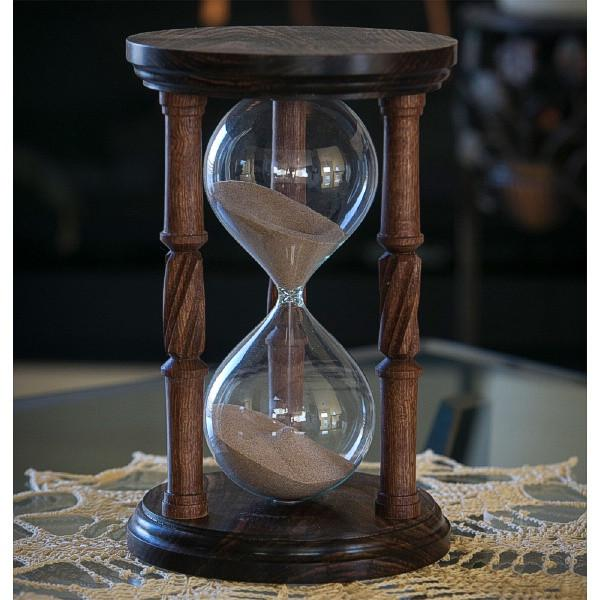
\includegraphics[width=0.4\textwidth]{figs/hourglass_whole.jpg}
  \caption{
    3D column collapse: a column collapse simulated with DEM (left) and with our hybrid method (right) at the same snapshots in time.
  }
  \label{fig:hybrid:column_collapse_3d}
\end{figure}

Extending to 3D, we also obtain a good qualitative matchup of the collapse in motion. Fig.~\ref{fig:hybrid:column_collapse_3d} shows the motion of a discrete and a hybrid column collapse.
Again note the grains at the edge of the runout, which the hybrid technique is able to capture.

\section{Silo Discharge}
In Fig.~\ref{fig:hybrid:silo_discharge}, we simulate a silo that discharges grains using a purely discrete approach and our hybrid approach.
With our approach, the oracle identifies the interior of the
initial mass of grains as a continuum. As grains exit the silo and the continuum region falls towards the orifice, our
method automatically converts the continuum material to discrete material. As grains form a pile on the ground, our
method detects the formation of the sufficiently dense portions of the pile and automatically converts discrete grains
to continuum material points in this area.

\begin{center}
  \centering
  \includegraphics[width=0.8\linewidth]{figs/silo_larger.pdf}
  %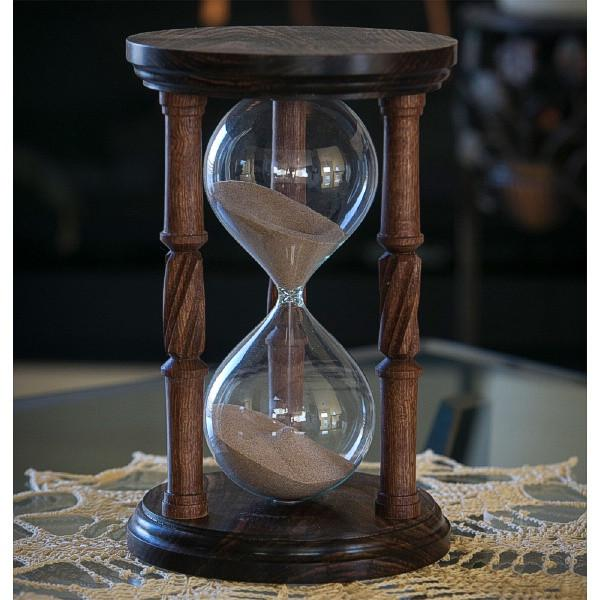
\includegraphics[width=0.4\textwidth]{figs/hourglass_whole.jpg}
  \captionof{figure}{
    Silo discharge: A silo discharges grains with a discrete method (left) and with our hybrid method (right).
  }
  \label{fig:hybrid:silo_discharge}
\end{center}

The hybrid 2D hourglass has a slightly faster flow rate than the discrete only counterpart. We believe that the ability to control the coordination number for newly sampled DEM particles would reconcile these flow rates. Generating packings given constraints is an interesting avenue of future work.

\begin{center}
  \centering
  \includegraphics[width=0.5\linewidth]{figs/bouncing_silo/hybrid/combine.pdf}
  %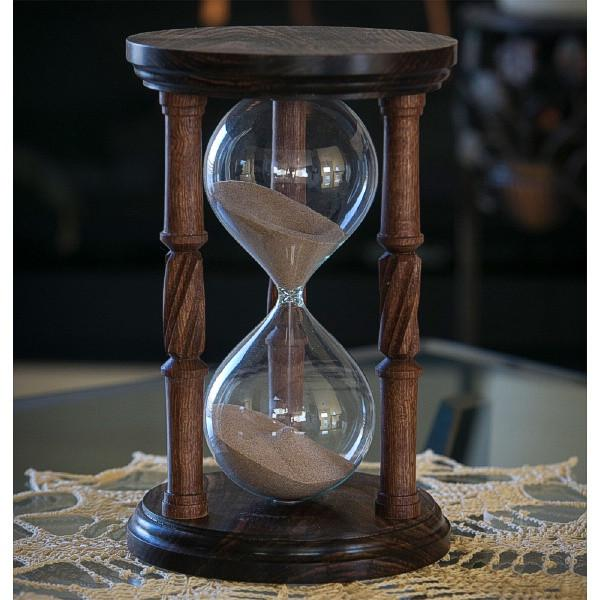
\includegraphics[width=0.4\textwidth]{figs/hourglass_whole.jpg}
  \captionof{figure}{
    3D silo discharge simulated with our hybrid approach: Left is a full view of the discharging grains while right is a cutaway view.
  }
  \label{fig:hybrid:silo_discharge_3d}
\end{center}

We also simulate a hybrid silo discharge in 3D (Fig.~\ref{fig:hybrid:silo_discharge_3d}). The hybrid approach is able to model ballistic motion and collisions after grains flowing from the silo enter a "gaseous" state. This ability to model contact is crucial for capturing the asymmetrical shape of the column, as well as the ballistic bounces when grains impact the container and the pile, both of which are observed in real-life hourglasses.
\begin{center}
  \centering
  \includegraphics[width=0.5\linewidth]{figs/bouncing_silo.pdf}
  %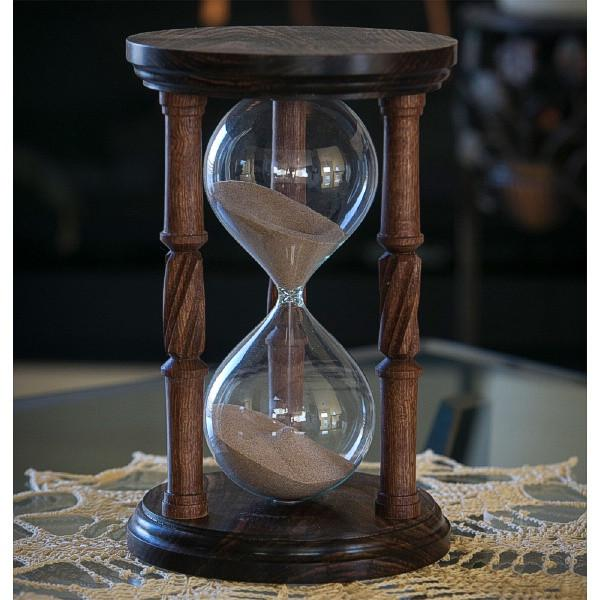
\includegraphics[width=0.4\textwidth]{figs/hourglass_whole.jpg}
  \captionof{figure}{Silo discharge (3D large orifice, $r=1.8$): Top: with $0$ restitution, the flow looks uniform. Middle: with $e=0.5$, the flow appears more energetic, with multiple fly away grains. The pure MPM version of this simulation (bottom) has a less energetic flow and fails to simulate grains bouncing away from the bulk.}
  \label{COR-compare}
\end{center}

MPM fails at simulating fly away grains, as the Particle-in-Cell method handles collisions by homogenizing each Lagrangian particle's velocity onto a background Eulerian grid and then transferring back. This series of operations results in an effectively inelastic collision among Lagrangian particles, i.e. with restitution coefficient $e = 0$. Note that this inelastic nature is independent of the particle-grid transfer scheme, i.e. PIC, FLIP, or APIC.

In contrast, our hybrid approach handles the full range of restitution coefficients from $0$ to $1$, due to the fact that we handle these collisions via DEM. In Fig.~\ref{COR-compare}, we show a comparison between $e=0$ and $e=0.5$. Note that the MPM counterpart is simulated with sticky boundary conditions on the bottom. Notice that when $e=0$, the hybrid approach results in the expected behavior of less energetic-appearing grains. It fails to capture the detailed bouncing effects and has a more uniform shape and flow profile.
\begin{center}
  \centering
  \includegraphics[width=0.8\linewidth]{figs/jamming.pdf}
  %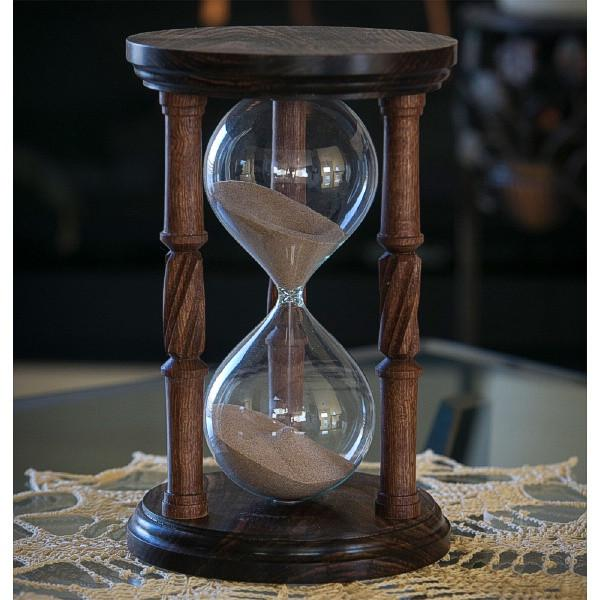
\includegraphics[width=0.4\textwidth]{figs/hourglass_whole.jpg}
  \captionof{figure}{
    Silo discharge (small orifice, $r=0.2$): A silo discharges grains with a discrete method (left), our hybrid
    method (middle), and a continuum method (right). Both the discrete and hybrid approach capture size-dependent clogging effects, and
    all flow from the orifice halts. The continuum simulation, in contrast, flows nonphysically.
  }
  \label{fig:hybrid:silo_frictoinal_jam}
\end{center}
Another advantage of our hybrid approach over a purely continuum method is the ability to frictionally
jam due to so-called finite size effects. In Fig.~\ref{fig:hybrid:silo_frictoinal_jam}, we simulate a silo discharge with a small orifice
width using a purely DEM algorithm, our hybrid algorithm, and a purely continuum algorithm. Note that we use an MPM cell width to DEM mean grain diameter ratio of 1:1 to more accurately couple the hybrid region near the orifice. Our hybrid simulation, like the purely DEM simulation, jams with the small orifice width, as expected. On the contrary the continuum, regardless of the grid resolution, fails to capture these finite size effects. Extra non-local modeling is needed \cite{Kamrin:2014}.

\section{Penetrometer Insertion}
\begin{figure}
  \centering
  \includegraphics[width=0.8\linewidth]{figs/stake_insertion.pdf}
  %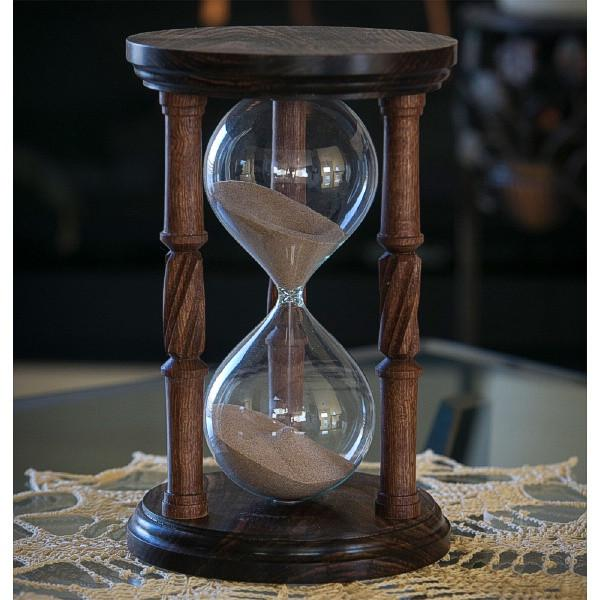
\includegraphics[width=0.4\textwidth]{figs/hourglass_whole.jpg}
  \caption{
    Penetrometer insertion: We insert a penetrometer into a bed of grains with our hybrid algorithm (first four frames).
    As the penetrometer enters the bed, our hybrid oracle identifies the region around the tip as requiring a discrete
    treatment and enriches the simulation domain in this area. As the simulation progresses, the continuum region
    eventually experiences a topology change and splits in two. Examining an overlay of a hybrid simulation (purple) on a purely discrete simulation (peach), we find the resulting profiles to be in almost perfect agreement (rightmost frame).
  }
  \label{fig:hybrid:stake_insertion}
\end{figure}

% \todo{{\bf Interaction with general rigid bodies}:
% Since our method uses discrete element to simulate grains on the free surfaces, it naturally handles interactions with general rigid bodies.}

Similar to Yan et al.~\cite{Yan:2010} and Wellmann and Wriggers \cite{Wellmann:2012}, we perform a hybrid
simulation of a penetrometer insertion into a bed of grains (Fig. \ref{fig:hybrid:stake_insertion}). These simulations
are difficult to perform directly with standard continuum methods owing to the massive plastic shape changes observed
around the penetrometer tip. Unlike previous works, we do not specify the region to be treated with DEM
a-priori. Instead, as the penetrometer advances into the bed of grains, our hybrid method is able to
enrich the region surrounding the penetrometer, ensuring that it always interacts with the bed through discrete grains.
As the penetrometer is fully inserted into the bed, the original single continuum region is split in two. Our hybrid
approach gracefully treats this topological change with no extra machinery.

\section{Bunny Toss}
\begin{center}
  \centering
  \includegraphics[width=0.4\linewidth]{figs/bunny_drill/toss_config_0032_COR00.pdf}
  \captionof{figure}{The bunny crashes into a container of gumballs with different coefficients of restitution using our hybrid method.}
  \label{fig:hybrid:bunny_toss}
\end{center}
We initialize a bunny with non-zero translational and angular velocity and simulate the resulting collision 
with a packing of gumballs. This high-speed bunny produces a splash upon impact with the gumballs before coming to rest.
In Fig.~\ref{fig:hybrid:bunny_toss}, the top simulation has zero restitution, while the bottom simulation has restitution of $e = 0.5$.
The larger coefficient of restitution leads to a simulation with a more dynamic splash.

While DEM uses 120,000 grains to simulate this scene, our hybrid approach only uses an average of 28,289 grains. In total, taking into account of the cost of MPM and the coupling computation (where again the MPM cell width is $2\times$ the mean grain diameter), our method is $1.74\times$ faster than DEM (Table \ref{tbl:speedup}).

\section{Excavator}
\begin{center}
\centering
  \includegraphics[width=0.4\linewidth]{figs/bunny_drill/excavator.pdf}
  %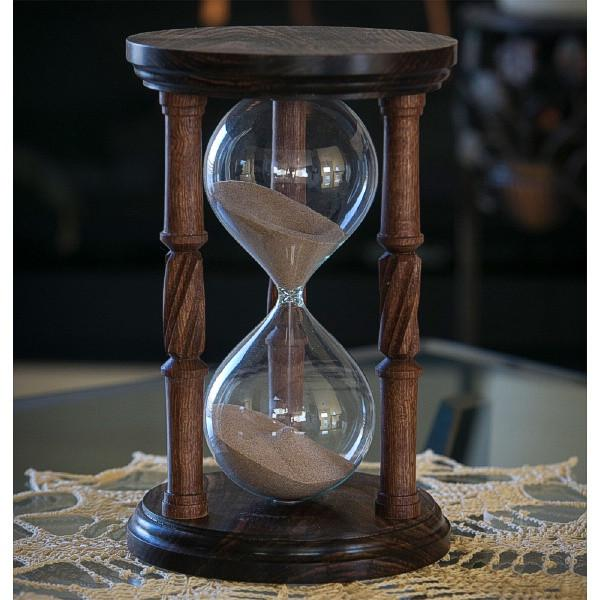
\includegraphics[width=0.4\textwidth]{figs/hourglass_whole.jpg}
  \captionof{figure}{We script an excavator to scoop gumballs out of a container.}
  \label{fig:hybrid:excavator}
\end{center}

In Fig.~\ref{fig:hybrid:excavator}, we script an excavator to scoop gumballs from the same container as the bunny toss. Our hybrid oracle robustly handles topology changes in the simulation domain induced by the excavator. Although not visible, as the excavator enters the granular pile, the continuum elements directly below the top DEM and hybrid layers are enriched to DEM grains. As the excavator digs in and rotates through the pile, it only interacts with DEM grains. material, it only  As we employ the same granular packing as the bunny toss in this test, we obtain a comparable speedup to that example.

\section{Bunny Drill}
 \begin{center}
 \centering
 \includegraphics[width=1.0\textwidth]{figs/bunny_drill.pdf}
 \captionof{figure}{Four rigid bunnies are scripted to rapidly rotate about the vertical axis while simultaneously moving into and out of a packing of 360,000 grains. The bunnies inject a large amount of energy into the system, causing significant displacement of grains in the interior while also producing an energetic splash near the free surface. From left to right we show: a cutaway view of initial conditions for a hybrid simulation, a cutaway frame from when the bunnies have penetrated the surface, a top down view of the same frame, and a cutaway view of purely discrete simulation at the same frame.}
 \label{fig:hybrid:bunny_drill}
 \end{center}
 
We aggressively insert and remove four scripted bunnies from a pile of 360,000 grains (Fig.~\ref{fig:hybrid:bunny_drill}). While initially only the top surface is represented as discrete grains, our method is able to dynamically enrich the interior around the bunnies in response to their motion. Our hybrid method obtains a similar visual result compared to the pure DEM simulation, yet it uses $88\%$ fewer discrete grains and is thus $6.82\times$ faster (See Table ~\ref{tbl:speedup}).

The bunny drill provides a key example of when the hybrid method is useful. While visually the only grains seen from the observer are the grains at the top of the container, the behavior of those flyaway grains are directly impacted by the physics of the granular layer underneath. By still solving for physics while the bunnies are not visible we enhance the final result, while still retaining a speedup over a pure discrete simulation that would capture similar visible granular dynamics. Also much like the excavator example, as the bunnies move through the interior of the domain, they are constantly kept in contact with discrete grains, so that any momentum transfers occur at bunny-DEM interfaces. This does away with the need to introduce continuum contact laws. Another advantage of the hybrid technique is thus shown: while we use the DEM to simplify the need to derive complicated constitutive laws in the continuum, we also use the DEM to simplify contact laws with rigid bodies.

\section{Tires on Gravel Road}
\begin{center}
  \centering
  \includegraphics[width=0.4\textwidth]{figs/bunny_drill/tire/config_0000_single_cropped.png}
  \includegraphics[width=0.4\textwidth]{figs/bunny_drill/tire/config_0066_speed_multi.png}
  \includegraphics[width=0.4\textwidth]{figs/bunny_drill/tire/config_0052_density.png}
  %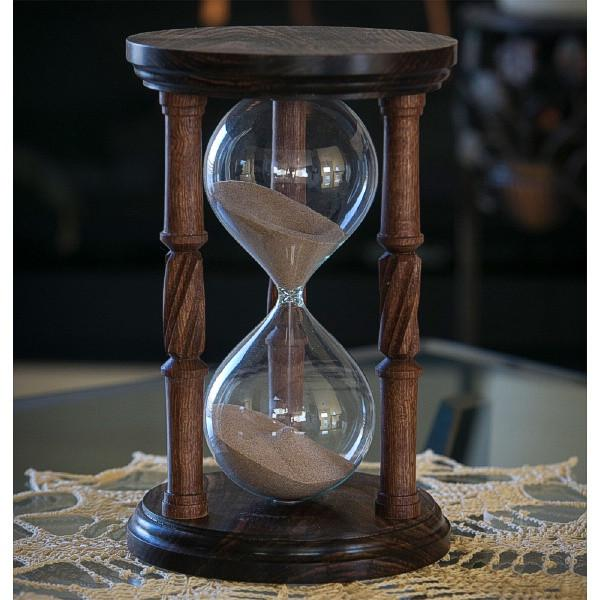
\includegraphics[width=0.4\textwidth]{figs/hourglass_whole.jpg}
  %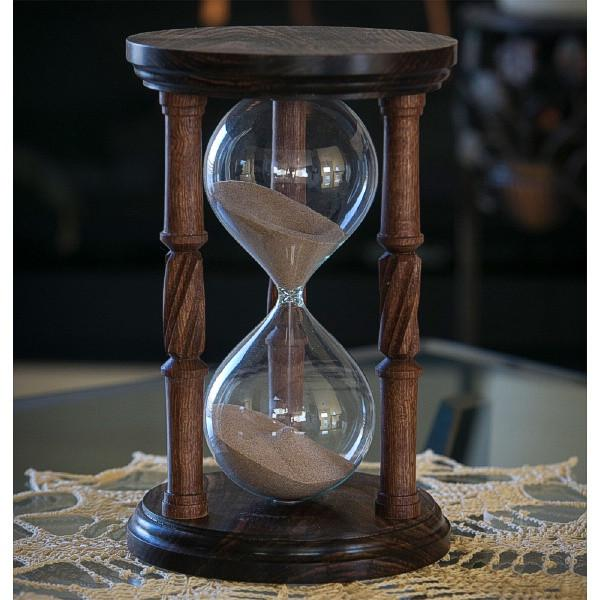
\includegraphics[width=0.4\textwidth]{figs/hourglass_whole.jpg}
  %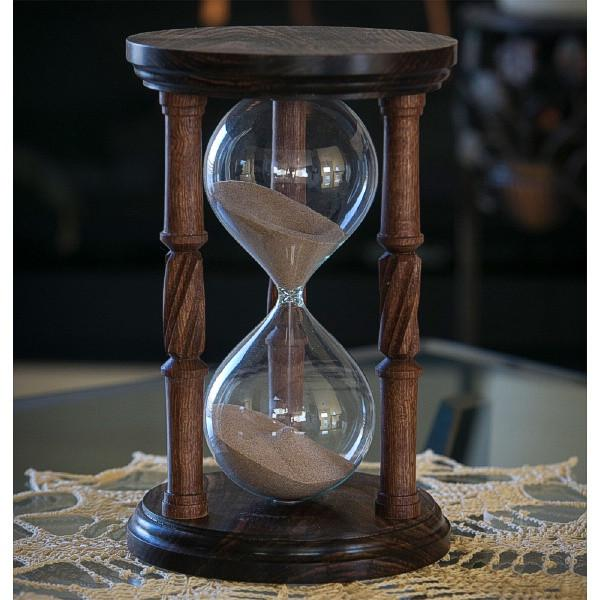
\includegraphics[width=0.4\textwidth]{figs/hourglass_whole.jpg}
  \captionof{figure}{Simulations of tires traversing a bed of gravel. Left: A render of the initial condition (boundary condition not shown), with a tire poised to race across the bed of grains. Notice the layered hybridization employed here. Center: Tires with different angular velocities but equal densities. Left to right the tires rotate at 1000 rad/s, 100 rad/s, and 10 rad/s. The 1000 rad/s tire produces a large granular splash while the 10 rad/s tire produces almost no splash. Right: Tires of different densities, but with the same angular velocities. Left to right the tires have $5\times$, $2\times$, and $1\times$ the density of gravel. As the tires traverse the system, the larger density tires sink into the gravel.}
  \label{fig:hybrid:tire}
\end{center}
On a slightly less whimsical note and to test our method on a more real world example, we simulate off-road tires traversing a gravel road. The tires are given a constant angular velocity around each of their axes, but are otherwise dynamically simulated. The hybrid method is able to capture multiple effects such as large splashes when fast rotating wheels collide with the grains, as well as tires sinking into the pile of grains due to a large density difference. While simulating this scene with a pure discrete method requires 822,956 grains, our hybrid approach allows us to simulate only a thin layer of discrete grains and the remainder is continuum (Fig.~\ref{fig:hybrid:tire} (a)). Here, the MPM cell width is $1.75\times$ the mean grain diameter. On average, the hybrid approach is $3.43\times$ faster than a purely discrete method (Table ~\ref{tbl:speedup}).

Again, as the tires dig through the domain, DEM grains are constantly being enriched, so that the entires only interact with those grains. The enrichment also provides a source for grains that are splayed back behind the tire.

\section{Spinning Drum}

\begin{center}
  \centering
  \includegraphics[width=0.8\linewidth]{figs/drum.pdf}
  %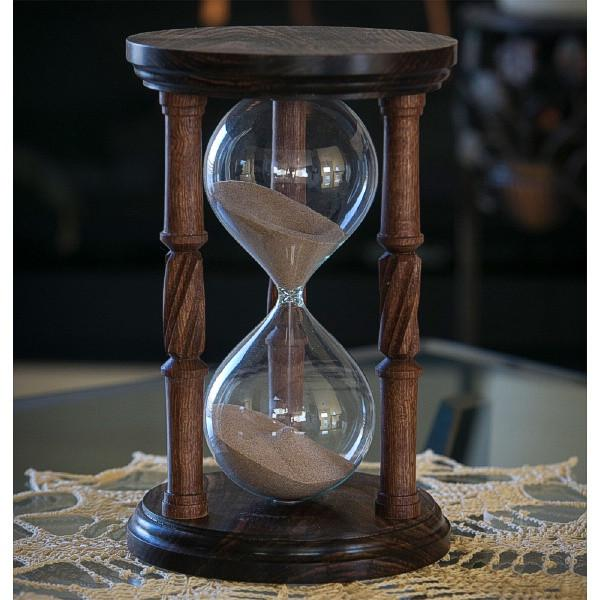
\includegraphics[width=0.4\textwidth]{figs/hourglass_whole.jpg}
  \captionof{figure}{
    Spinning drum: We rotate a drum filled halfway with grains using DEM (top row) and using our
    hybrid algorithm (bottom row). As the system evolves, observe that the shape of the free surface obtained with our
    hybrid method agrees with that of the purely discrete method.
  }
  \label{fig:hybrid:spinning_drum}
\end{center}

Continuing the theme of more practical applications, we simulate the flow of grains in a spinning drum. An understanding of drum geometries is important in industrial applications (e.g. mills,
tumblers) and in the study of free-surface flows \cite{Midi:2004:Dense}. To assess whether our algorithm is
suitable for these geometries, we fill a drum with grains to half its area, and impose a rotation to the drum with
a constant angular velocity.

With a pure DEM simulation, we observe nearly rigid grains near the base of the drum, a steadily increasing flow towards the interior of the granular assembly, and loosely packed grains near the free surface. As the transient phase subsides, we observe the characteristic free-surface shape. Our pure DEM simulation thus matches physical experiment and other numerical simulation, providing a baseline of comparison.

Thus comparing the purely discrete results to those from our hybrid algorithm (Fig.~\ref{fig:hybrid:spinning_drum}), we find
the profiles to be in good agreement throughout the simulation. Because our hybrid algorithm treats
regions near surfaces with discrete grains, we do not require any additional machinery to handle the drum boundary
condition beyond that from the discrete simulation. Again, we demonstrate the advantage of the hybrid algorithm in treating interactions with boundaries and rigid objects. Like the discrete simulation, our hybrid algorithm is also able to
capture free flight fly away grains near the top of the domain.

\section{Speedup Study}
\begin{center}
  \centering
  \includegraphics[width=0.6\linewidth]{figs/chute_flow.pdf}
  %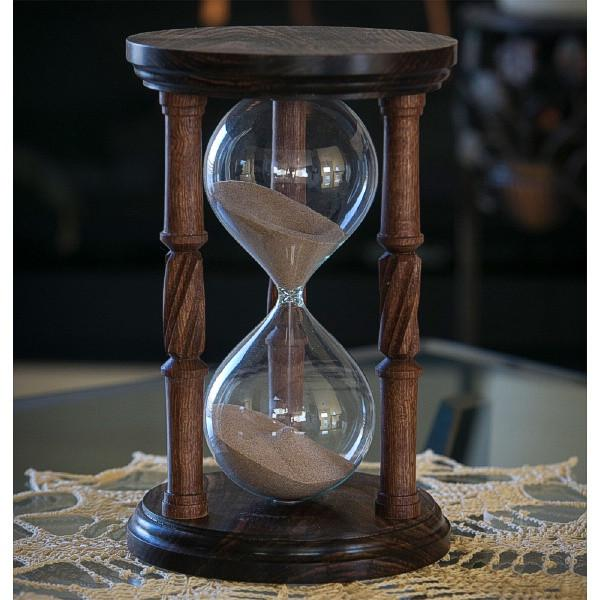
\includegraphics[width=0.4\textwidth]{figs/hourglass_whole.jpg}
  \captionof{figure}{
    Periodic chute flow: We set a granular packing at an angle $\theta$ with periodic boundary conditions to simulate flow down a chute.
  }
  \label{fig:hybrid:chute_flow}
\end{center}

We seek to quantify the speedup we are able to obtain from the hybrid
method over a pure discrete simulation. In order to do this, we use the geometry, seen in
Fig.~\ref{fig:hybrid:chute_flow}. Grains are initialized in a column and are then tilted at an angle $\theta$ relative
to the horizontal, with gravity applied. We then apply periodic boundary conditions, causing a continual 
flow of grains down-slope. Three factors are adjusted: the initial total number of grains $N_i$ before hybridization, the fraction of DEM left
after the hybridization $F$, and the hybrid grid size (identical to the MPM grid size here) $H$. A parametric sweep
over these variables allows for the construction of a phase plot, which shows for a given $N_i$, when a 
pure discrete simulation with $N_i$ grains is faster or slower than a hybrid simulation initialized with $N_i$ grains but with
different $F$ and $H$. Note that the geometry is kept fixed for all simulations, so that increasing or decreasing $N_i$ means
decreasing or increasing the average grain diameter.

\begin{figure}
  \centering
  \includegraphics[width=0.75\linewidth]{figs/phase_plots2.pdf}
  %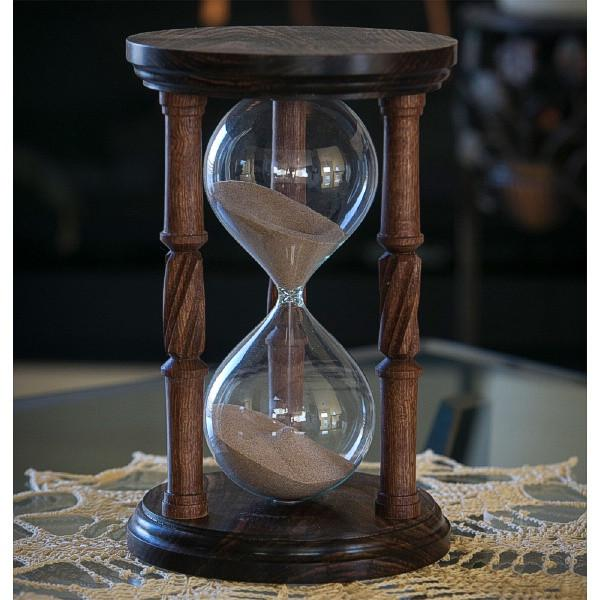
\includegraphics[width=0.4\textwidth]{figs/hourglass_whole.jpg}
  \caption{
    Phase plots: Phase plots for $H = 0.0025$ (top left), $H = 0.00125$ (top right), $H = 0.00083$ (bottom left), and $H = 0.000625$ (bottom right). Red denotes
    regimes where our hybrid scheme is faster while blue denotes regimes where DEM is faster.
  }
  \label{fig:hybrid:phase_plots}
\end{figure}

$N_i$ ranges from 1,000 grains up to 156,000 grains, $F$ ranges from $0.07$ to $0.89$, and $H$ ranges from $0.0025$ to $0.000625$. Cell width to mean grain diameter ratios thus range from 19:1 to 0.4:1.
Fig.~\ref{fig:hybrid:phase_plots} displays phase plots over different values of $H$. As $H$ decreases, more elements are hybridized, and so computational costs associated
with hybridization increase. However, even for the most refined grid, a speedup can still be obtained with a reasonable $F$ for a simulation requiring 40,000 grains or more.
It can be seen from Fig.~\ref{fig:hybrid:phase_plots} that a speedup on the order of $12\times$ can be obtained. While it may seem that increasing the resolution (thus decreasing $H$)
results in a decay of the maximum speedup obtained, one can exploit a characteristic of a smaller $H$: with smaller $H$, a smaller $F$ can be obtained.

Looking at the relationship between $H$ and $F$ from a different perspective, an analysis of the speedup for layered hybridization in 2D can be conducted from the geometry of the problem. Letting $C_D$ be the computational cost
of a discrete grain, $C_E$ the cost of enrichment for a hybrid cell, $C_C$ the cost for a continuum element, and $A$ the effective total number of grains (average number of grains per 
cell multiplied with the number of cells containing grains), we obtain the following expression for the total time $T_H$ for a complete hybrid iteration and total time $T_C$ for a pure discrete simulation:

\begin{align}
\begin{aligned}
T_H &= C_EhN^2 +C_D\frac{(N_D+N_H)N}{hN^2}+C_C(hN-N_D)N , \\
T_C &= C_DA.
\end{aligned}
\end{align}

A reduction ratio $R_A$ can then be defined between the computational time of a hybrid simulation and an equivalent discrete simulation of $A$ grains:

\begin{align}
R_A &=\frac{T_H}{T_C}=\frac{C_E h N^2}{C_DA} +\frac{C_D (N_D+N_H)N}{hN}+\frac{C_C (hN-N_D)N}{C_DA}.
\end{align}

Minimizing $R_A$ results in the largest speedup, 
and we can find the optimal $N$ giving the largest speed up as:
%and it can be shown that $R_A$ can be written as:
\begin{align}
\begin{aligned}
%R_A &=\frac{C_E}{h(C_E+C_C)N}+\frac{2}{hN} +\frac{C_C}{h^2(C_E+C_C)N}\left(h-\frac{1}{N}\right) \\
N & = \left(\frac{C_DA}{h^2(C_E+C_C)}\right)^{1/3}.
\end{aligned}
\end{align}

The key insight is that if $N$ is chosen in the manner shown above in relation to $A$, then as $A\rightarrow\infty$, $R_A\rightarrow0$, which means that increasing speedups
can be had for increasing grain numbers. This is an extremely useful property, and serves to highlight the potential of our hybrid method to tackle problems bridging 
micro/mesoscale causes to macroscale effects. 

For the layered hybridization method in 3D described in Section~\ref{sec:layered_3D}, we obtain the best speedups if $N$ scales with $A$ according to $N \propto A^{1/4}$. Then as $A\rightarrow\infty$, $R_A\rightarrow0$.

It is important to note that $N$ scales with $A$ in the power of $1/4$ ($1/3$ in 2D), not $1/3$ ($1/2$ in 2D).
An intuitive explanation is that if we refine both the discrete and continuum elements equally (this corresponds to setting $N \propto A^{1/3}$ ($N \propto A^{1/2}$ in 2D)) while keeping the discrete layer thickness to a minimum,
then the discrete computation time will scale as $N^2$ ($N$ in 2D) whereas the
continuum will scale as $N^3$ ($N^2$ in 2D), so eventually the continuum computation time will dominate, and we
will hit a bound. However, if we refine them \textit{differently} and maintain a balance between the two (i.e., setting $N \propto A^{1/4}$ in 3D and $N \propto A^{1/3}$ in 2D),
then the acceleration continues.

\section{Core Scaling}
\begin{figure}
  \centering
  \includegraphics[width=0.5\textwidth]{figs/core_scaling.pdf}
  %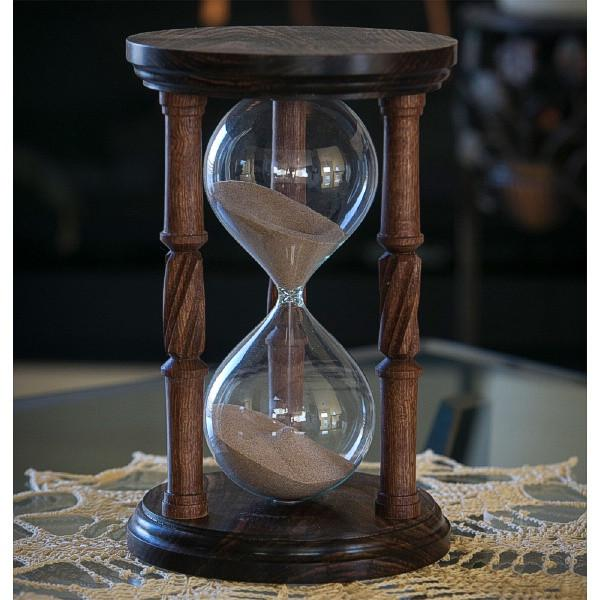
\includegraphics[width=0.4\textwidth]{figs/hourglass_whole.jpg}
  \caption{
    Periodic chute flow: We set a granular packing at an angle $\theta$ with periodic boundary conditions to simulate flow down a chute.
  }
  \label{fig:hybrid:chute_flow}
\end{figure}


It should be noted that while the hybrid technique itself is able to push the domain sizes we are able to simulate, the ability to run in parallel is also crucial for even larger problems. Therefore we require an analysis of how well the code scales with core count.

To study how well our code parallelizes, we conducted a test with the bunny drill example. We ran both a pure DEM and a hybrid simulation of the bunny drill with varying core counts. For each core count, we ran each simulation for two hours of wall clock time and measured the number of completed time steps. 

As evident from Figure \ref{fig:hybrid:chute_flow}, both DEM and our hybrid method do parallelize, albeit with sub-linear scaling. We note that at the time of this test, many routines in the code were not fully parallelized, and a complete refactoring with parallelization in mind would greatly improve scaling. For example, a domain decomposition algorithm across all components of the hybrid solve would result in much closer to linear scaling.




%% This is an example first chapter.  You should put chapter/appendix that you
%% write into a separate file, and add a line \include{yourfilename} to
%% main.tex, where `yourfilename.tex' is the name of the chapter/appendix file.
%% You can process specific files by typing their names in at the 
%% \files=
%% prompt when you run the file main.tex through LaTeX.
\newcommand\mystrut{\rule[-0.9cm]{0pt}{2cm}}


\chapter{Enrichment and Homogenization Improvements}
The Results section showed that, for the problems run, the implementation of the hybrid method seems adequate to capture bulk behavior, like the end shape of a pile of collapsed grains. This however is interesting, as the previously described scheme includes a somewhat straightforward solution to ill-posed problems. The most ill-posed portion of the hybrid technique is the enrichment step, as a given continuum state can be represented by an infinite set of discrete element grain arrangements.

The solution applied to the enrichment problem, Avoid a Void, simply adds grains to all hybrid elements. There is no other information used to inform where Avoid a Void should place grains (as the Poisson Disk Sampling is random by nature), how many grains to add, or what kind of connectivity with other grains should be had. In the examples shown in the Results section, this is seemingly enough, as there are actually a relatively low number of conversions from discrete to continuum and continuum to discrete representations. For example, in the column collapse case, the core of the columns remain relatively steady, and conversion only happen around the exterior of the columns. Once the pile has collapsed, the pile remains steady and no other conversions occur. In the wheels driving over gravel example, there are also a lack of many conversions, as those conversions only occur for the elements directly under the wheel; once the wheel has driven past a set of elements, the granular bulk remains steady and the representations of the grains do not change.

The funnel flow example however indicates where the simple uninformed Avoid a Void scheme for enrichment can begin to break down. As can be seen in Figure \ref{fig:hybrid:silo_discharge}, the top half of the funnel starts with both the pure discrete and hybrid funnels at the same volume. However after some of the grains have flowed from the top half of the funnel to the bottom half, it can be clearly seen that the hybrid funnel flows at a different rate than the discrete grains. A key difference between the funnel flow geometry and the other previously discussed examples is that in the funnel flow, there is a continuous change from continuum to discrete grains at the top, and discrete to continuum grains at the bottom. The result is that the deficiencies of the enrichment and homogenization schemes are exposed. 

\section{Volume Change and Mass Conservation}
Every hybrid update step, the Avoid a Void scheme attempts to pack in grains in the hybrid elements. Because it does so in an uninformed matter however, this can lead to mass and volume loss or gain. For example, If the discrete grains in a hybrid cell have a large enough packing fraction $\Phi$ where the element remains hybrid, but below random close packing $\Phi_{RCP}$, the previously described enrichment scheme has a chance to pack in additional points. If that relatively low packing fraction is an accurate representation of the granular system at that element, then there may be mass introduced. If that hybrid element then is converted into a pure discrete element, permanent volume gain is then introduced into the system. 

On the other hand, mass can also be permanently lost in the system. If for a given hybrid element, the discrete grains have a packing fraction $\Phi < \Phi_{actual}$ based off of mass and volume that needs to be converted from a continuum representation, then the idea is that the Avoid a Void algorithm will eventually fill that missing space. However, Poisson Disk Sampling (PDS) has a limit and will not be able to reach $\Phi_{RCP}$. If $\Phi_{actual} \approx \Phi_{RCP}$ or worse, if $\Phi_{actual} \geq \Phi_{RCP}$ because the underlying discrete structure is crystalline, PDS will not be able to pack that space to the desired $\Phi$. In some geometries and flows, this may not be a problem, as, if the conversions happen at a slow rate compared to the hybrid update frequency, then the grains in an underpacked hybrid cell may rearrange to allow for PDK to pack in the enough grains. The column collapse and wheel examples for example, fall under this category. The funnel flow however has a continual flux of continuum into the hybrid zone which must be enriched. Mass loss occurs because the continuum to enrichment mass flux is larger than the source of discrete hybrid mass that the enrichment scheme can provide. The resulting lack of discrete particles then leads to volume loss.

\begin{figure}[htp] 
    \centering
    \subfloat[]{{\includegraphics[width=0.3\textwidth]{figs/paraviewSetup/chute_initial.png} }}%
    %\qquad
    \subfloat[]{{\includegraphics[width=0.3\textwidth]{figs/paraviewSetup/chute_0_5s.png} }}%
    %\qquad
    \subfloat[]{{\includegraphics[width=0.3\textwidth]{figs/paraviewSetup/chute_1s.png} }}%
    \caption{Evolution of a hybrid flow down a chute showing mass loss. (a) Initial state. (b) After 0.5s of flow. (c) After 1s of flow.}%
    \label{chute_flow_old}
\end{figure}

As an extreme example, take the example of a flow down a chute with periodic boundary conditions. In this system, gravity is angled relative to the bottom boundary, driving continuous flow through the system. On the left side. discrete grains continuously enter a hybrid zone, where continuum points are in turn generated. As they move from left to right through the system, the discrete points are deleted as they enter the pure continuum zone and continuum points gain full weightage. The points then enter the hybrid zone on the right, where discrete grains are generated. Finally the continuum points exit into the discrete zone where they are deleted, and the discrete grains gain full weightage. With the current scheme, mass and volume are continuously lost. Eventually the pile of flowing grains reduces to a point where there is insufficient height to support a continuum or hybrid scheme according to the oracle, resulting in a pure discrete system.

There are thus two main problems that must be addressed: mass conservation and volume change tracking. These two problems however must be resolved in the discrete representation and continuum representation in different ways. Mass conservation for the continuum representation (converting mass from discrete grains to continuum) is fairly simple, as the continuum nature allows for mass addition or subtraction in whatever increments desired. Mass in the continuum can thus be tracked exactly over time. Volume change though must be conducted in a manner consistent with that mass change, and this must be addressed. 

For the discrete representation, mass conservation and volume change are completely coupled, as the density of the particles remains constant throughout the simulation. Mass conservation is more difficult to achieve in the discrete case, as mass conservation becomes a packing problem as previously described. Mass and volume in the discrete case also come in discrete units of a single grain at a time. This means that mass conservation cannot be exactly achieved in the discrete representation. The homogenization of a grain of radius $r_a$ can be offset by the enrichment of a grain of radius $r_b$, but mass will only be exactly conserved if $r_a = r_b$. For a monodisperse system this will of course always be true, but all the simulations run in this study have some polydispersity, making that condition almost never true. Thus mass conservation can only be achieved in a time-averaged sense for the discrete particle representation.

\subsection{Mass Ledger}

\begin{figure}[htp] 
    \centering
    \includegraphics[width=0.8\textwidth]{figs/simple_hybrid.pdf}
    \caption{Mass fluxes in a hybrid system.}
    \label{mass_ledger_schematic}
\end{figure}

In order to conserve mass and inform the enrichment scheme on how much mass must be converted from one representation to another, all of the relevant mass fluxes must be kept track of. Take as an example the simple hybrid system shown in Figure \ref{mass_ledger_schematic}. Again, a simple 50/50 weight split in the hybrid system is shown both for simplicity and to reflect the weight function used in the current study. At the $n^{th}$ hybrid update, the marked DEM grain has radius $r_d$, density $\rho_d$, and weight $w^n_d=1$, resulting in a mass $m^n_d=m_d=w^n_d\rho_d\pi r^2_d$. At the $n^{n+1}$ hybrid update, the discrete grain $d$ has moved into the neighboring hybrid element (Element 1). Now, $w^{n+1}_d=0.5$, resulting in a mass $m^{n+1}_d=1/2m^{n}_d$. The mass difference $\Delta m_d=1/2m^d$ is mass that must be represented by continuum in order to maintain a partition of unity for the total mass that entered, $m_d$. There is thus a \textit{deficit} of continuum mass in Element 2 that must be added, through addition of mass to the currently existing MPM points, addition of a new MPM point with that deficit, or some combination of both.

Moving attention to the marked MPM point, the MPM point $p$ at the $n^{th}$ hybrid update is in the hybrid zone and has weight $w^n_p=0.5$ and mass $m^n_p=w^n_p m^p=0.5m^p$. At the next hybrid update its weight changes to 1, resulting in a mass of $m^{n+1}_p=m^p$ and a resulting continuum mass \textit{excess} in Element 3 of $0.5m^p$. 

From these cases it can be seen there are multiple ways that discrete and continuum mass can accrue deficits or excesses depending on weight changes as they move between different zone types. These excesses or deficits are logged in a mass \textit{ledger}, which informs the enrichment and homogenization schemes on how much mass of which type of representation is required. It should be noted that while there must always be at least one hybrid zone between a pure discrete and pure continuum zone, we still account for the rare chance that a grain in a pure discrete zone at hybrid update step $n$ advects to a pure continuum zone by hybrid step $n+1$ due to geometry and hybrid update frequency.

This case is not treated any differently to the previously described cases. While the discrete point is deleted from the system for being in a pure continuum zone, this can be interpreted as simply a weight change from $w_d=1$ to $w_d=0$. This results in a continuum mass deficit of $m_d$ in the element that the grain was deleted from. The same could of course occur for an MPM point entering a pure discrete region, resulting in a discrete mass deficit.

This analysis so far has assumed a fixed domain decomposition, where all element types remain fixed over time. This however does not need to be the case, as the framework of mass deficits or excesses as a result of weight changes can generalize to a system where DEM grains and MPM points advect through elements with different representations, as well as the representations themselves changing from timestep to timestep. For the mass ledger, all that needs to be known is the type of zone that the grain or point was in at the previous hybrid update, and what type of zone it is currently in. If the zone type was the same for the starting element at the previous update as the current element at the current update, then no change to the ledger needs to be made. If the zone types are different, then the mass difference due to the weight change is then marked in the ledger.

\subsection{Mass Ledger Implementation}
In order to keep track of mass deficits or excesses, two ledgers are introduced, which, in implementation, are simple vectors: the \textbf{dem\_deficit} and \textbf{continuum\_deficit}. Each vector stores the eponymous mass deficit on each element in the simulation. To establish convention, mass deficits are positive and excesses are negative. Assuming an MPM point starting with a mass $m_p$ and a DEM grain with mass $m_d$, the ledger changes can be summarized as:

\def\Zones{\makecell[tl]{Discrete\\ Continuum\\ Hybrid\\ \\ Discrete\\ Continuum\\ Hybrid}}
\def\demdeficit{\textbf{dem\_deficit}}
\def\mpmdeficit{\textbf{mpm\_deficit}}

\begin{table}
  \centering
  \footnotesize
  \renewcommand{\cellalign}{lc}
  \begin{tabular}{lllll}
    \toprule
    Representation & Start Zone & End Zone & Ledger & Deficit  \\
    \midrule
    DEM Grain & \makecell[tl]{Discrete\\ \\ \\ \\Hybrid} & \Zones & \makecell[tl]{N/A\\ \mpmdeficit\\ \mpmdeficit\\ \\ \mpmdeficit\\ \mpmdeficit\\ N/A} & \makecell[tl]{N/A\\ $+m_d$\\ $+0.5m_d$\\ \\ $-0.5m_d$\\ $+0.5m_d$\\ N/A} \\
    \midrule
    MPM Point & \makecell[tl]{Continuum\\ \\ \\ \\Hybrid} & \Zones & \makecell[tl]{\demdeficit\\ N/A\\ \demdeficit\\ \\ \demdeficit\\ \demdeficit\\ N/A} & \makecell[tl]{$+m_p$\\ N/A\\ $+0.5m_p$\\ \\ $+0.5m_p$\\ $-0.5m_p$\\ N/A} \\
    \bottomrule
  \end{tabular}
  \caption{Mass ledger contributions.}
  \label{mass_ledger_table}
\end{table}

The mass ledgers for a hybrid update are calculated near the beginning of the hybrid update: it is done after the level set calculation and after the oracle has determined the zone types based on those calculations, but before the enrichment and homogenization steps. The ledgers are updated every hybrid update, so that there is a running list of mass deficits. This thus enables a way to prevent mass gain and tackle mass loss. If an element has a negative deficit due to, for example, introducing a grain with a slightly larger radius than was needed, then the ledger can inform the enrichment scheme to not introduce any more DEM grains in that cell. On the other hand, if there is a positive deficit, then if at a given hybrid update the packing scheme is unable to introduce enough grains, then there is a chance in future updates that the grains have reached a configuration to allow for further grain introduction. Implementation wise, only elements that have a positive deficit are marked for enrichment.

\section{Packing Schemes}
Practically speaking, the mass ledger mostly addresses mass gain problems, as it stops enrichment in those elements. In elements that have a deficit, the enrichment scheme will continuously try to input grains and points, but this is not any different than the previously used scheme which tried to pack grains for all hybrid elements at every hybrid update. The problem remains that for certain geometries and flow profiles, the Avoid a Void's PDS scheme, which is random in nature, was unable to introduce DEM grains at a high enough packing fraction at a rate equal to or greater than the continuum mass flux into a hybrid cell. A new packing scheme is needed. The following section summarizes the different packing strategies that were attempted and discusses their characteristics.

In order to evaluate the effectiveness of new packing schemes, the inclined plane geometry shown in Figure \ref{chute_flow_old} is used as a case study. The hyperelastic model was used to obtain the result shown in Figure \ref{chute_flow_old} for demonstration purposes; a switch is now made to the hypoelastic model, as it includes the $\mu(I)$ relation that captures the correct velocity profile in an inclined chute flow, minimizing the role of the constitutive law in the mass loss issue.

\subsection{Random Packing}
Before any new packing methodologies are introduced however, it should be noted that the random scheme has a parameter \textit{numTrials} which controls the number of attempts the code makes to introduce a new point. For all of the simulations shown in the Results section, this was set to 20, mostly as a compromise between speed and accuracy for the geometries that we. The first logical attempt at a solution to the packing problem is then to simply increase the number of attempts, trading the time lost in increasing the number of attempts for better packing. 

%\begin{figure}[htp] 
%    \centering
%    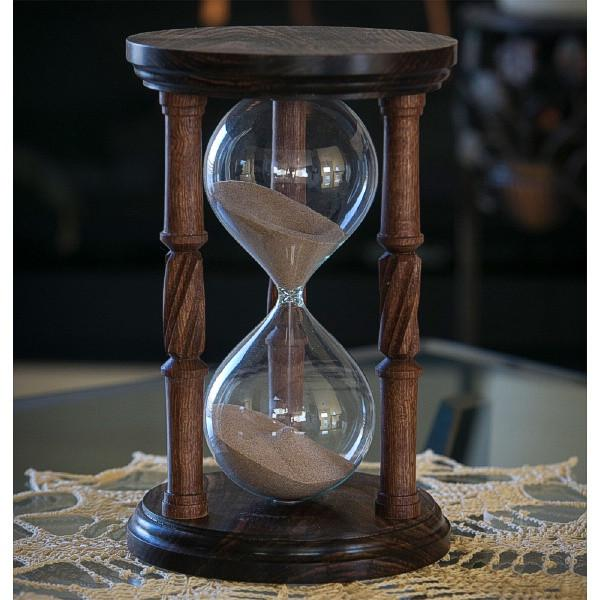
\includegraphics[width=0.4\textwidth]{figs/hourglass_whole.jpg}
%    \caption{Mass over time for random packing.}
%    \label{mass_time_random}
%\end{figure}
%As Figure \ref{mass_time_random} shows, this is not enough. 
While increasing \textit{numTrials} does help slow down the mass loss rate, the mass loss rate does reach a limit as a function of \textit{numTrials}. At first pass this may seem counterintuitive, as in the limit of infinite trials a dense configuration should be sampled. However, this is not true do the fact that the random packing scheme is a greedy scheme. If the random scheme picks a point center with a random radius that has no collisions with any other point in the enriched element, then that point will be considered valid and added to the existing points. This limits the possible areas that new grains can now enter, as can be seen in Figure \ref{greedy_dem}. 

\begin{figure}[htp] 
    \centering
    \subfloat[]{{\includegraphics[width=0.3\textwidth]{figs/non_optimal_packing_1.pdf} }}%
    %\qquad
    \subfloat[]{{\includegraphics[width=0.3\textwidth]{figs/non_optimal_packing_2.pdf} }}%
    %\qquad
    \subfloat[]{{\includegraphics[width=0.3\textwidth]{figs/non_optimal_packing_3.pdf} }}%
    \caption{Non-optimal enrichment. (a) Element that needs additional discrete grains. (b) Optimal packing that reaches desired packing fraction. (c) Actual sub-optimal placement of grain that prevents other grains (light blue) from being injected.}%
    \label{greedy_dem}
\end{figure}

\subsection{Grid Packing}
Enrichment can occur often, depending on the geometry of the problem. Because of this, speed is still a requirement of any practical packing scheme. Thus, while less informed greedy schemes may not provide adequete packing, they do potentially show a much larger speed advantage over other schemes. Packing in general is a problem that shows up in many contexts, and solutions do exist that show the ability to attain very high packing fractions that still avoid crystalline packings %\textcolor{red}{FINDREFERENCE}
. However these solutions are currently avoided, due to their computational expense. For example, some class of solutions solve a constrained minimization problem, maximizing packing fraction while constrained to limited or no overlaps. Introducing an optimization solve is potentially too slow for the current application. On the other hand there are a class of solutions that essentially inject grains at random in a system and substep a discrete element method to attain a viable configuration. Again, solving a sub discrete element problem with multiple timesteps needed to achieve an equilibrium state is too expensive.

Therefore, a more guided greedy method is desired. From Figure \ref{chute_flow_old} it can be seen that as the grains flow from left to right, space intuitively opens up upstream of the hybrid elements. The next solution attempted utilized this fact, prioritizing grain injection attempts to the downstream-most available spaces in the element, to promote closer packing to the currently existing grains. To do this, the area of an enriched hybrid element was discretized into a grid. The nodes of the grid represent possible injection points. As a note, this presents a parameter that must be tuned: the discretization distance between nodes. Smaller discretizations can lead to less space between injected points, but also increases the number of attempts that must be made. 

\begin{figure}[htp] 
    \centering
    \includegraphics[width=0.8\textwidth]{figs/grid_packing_scheme.pdf}
    \caption{Grid enrichment scheme.}
    \label{grid_enrichment}
\end{figure}

The scheme would then attempt to inject grains, starting from the downstream side. The downstream direction was determined by checking the surrounding elements of the element currently being enriched; if a continuum element neighbors the hybrid element, then the downstream element side is the side opposite of the shared element side. If a discrete element is adjacent to the enriched element, then that face is taken as the downstream side. If only hybrid elements surround the current element, then a direction is picked at random. 

\subsection{Circle Sweep}
\def\seed{\textbf{seed\_queue}}
While the grid scheme was an improvement over the initial random packing, it proved to still be unable to provide a discrete mass source that offset the continuum mass flux into a hybrid cell. The goal of the scheme was to increase the chances of introducing points closer to the existing points; this was achieved, but not to the desired level. To address this deficiency, the next scheme, deemed here the "circle sweep" scheme, strictly forced at least one point of tangency for any injected grain to the other grains in the cell.

\begin{figure}[htp] 
    \centering
    \includegraphics[width=0.5\textwidth]{figs/circle_sweep_scheme.pdf}
    \caption{Circle sweep scheme. (a) Initialize with seed grain (light blue). (b) Sweep around seed grain. (c) Move to the next seed in the queue. (d) Sweep around new seed grain.}
    \label{circle_sweep_enrichment}
\end{figure}

In order to discuss the scheme, take as an example a pure continuum element that at the current hybrid update is now a hybrid cell, and must be enriched. To initialize the scheme, a grain is injected at a random location within the element and is given an index number $i$ of 1. This index number is added to a queue of indices called the \seed. The angular arc of 2$\pi$ around this grain is then discretized into $n$ angular divisions. Grains injections are then attempted at all of these angular divisions at a distance equal to the sum of the radius of the seed grain $r_i$ and the new grain $r_{new}$, assuring that any new grain has at least one point of tangency to other grains in the element. A new valid grain is given an index number of 1 plus the index number of the grain at the rear of the queue, which itself is then enqueued. Once injection attempts have been made at all of the possible angles around the seed grain, the index of the seed grain is dequeued. The next grain in the \seed then becomes the seed grain, and the process is continued. The scheme then stops once the queue is empty.

In hybrid elements with DEM grains already present, the circle sweep algorithm begins by enqueueing all of those grains in the \seed, instead of injecting a grain at random to initialize the queue. The algorithm then continues as stated, working through the \seed. Again, this scheme introduces a tunable parameter $n$, which controls the number of injection attempts made around every seed grain.

\subsection{Two Point Tangent}
The circle sweep scheme represents an improvement over the grid scheme, but again, for the chute flow geometry was not enough to offset the continual continuum mass flux into the hybrid elements. The final scheme attempted, called the "two-point-tangent" (TPT) scheme, as its name suggests, enforces two points of tangency for any new injected points. 

\begin{figure}[htp] 
    \centering
    \includegraphics[width=0.5\textwidth]{figs/two_point_tangent.pdf}
    \caption{Two Point Tangent Scheme. (a) Initialize with seed grain (light blue) and  partner grain (green). (b) Inject new points at locations that are tangent to seed grain and partner grain. (c) Move to the next partner grain in the queue. (d) Inject any possible grains between the seed and new partner grains.}
    \label{two_tangent_enrichment}
\end{figure}

In order to initialize the TPT scheme for a newly enriched element, a grain is injected at random and added to the same \seed data structure as the circle sweep scheme. The angular region around the grain is again discretized and grain injections are attempted at these angles. The divergence point between TPT and the circle sweep scheme occurs when a valid grain is found and added to the \seed. Instead of continuing injection attempts at the other remaining possible angles, the scheme stops, and uses these two grains as the starting point of the scheme, with the first designated as the seed grain and the second as the partner grain. With these two tangent grains of radius $r_a$ and $r_b$, a new grain with radius $r_c$ can be injected that is tangent to both of the first two. Given the center points of the grains $a$ and $b$ and their radii, and the radius of the new grain $r_c$, an analytical formula can be derived for the two possible center points of the new grain $c$ that maintains tangency with $a$ and $b$. Injection attempts are then made at these two locations, and any valid attempts are added to the simulation and to the \seed. The partner grain then moves through the queue (without a dequeue operation), with any possible injection points between the seed and partner grains injected. Once the partner grain has gone through the entire queue, the seed grain is dequeued and moves to the next grain in the queue.

\subsection{Packing Scheme Results}

\begin{figure}[htp] 
    \centering
    \includegraphics[width=0.7\textwidth]{figs/compare_technique_m_v_t.pdf}
    \caption{Comparison of Normalized Mass vs Time for different packing techniques.}
    \label{packing_compare}
\end{figure}

Figure \ref{packing_compare} shows the normalized mass (mass of the DEM + MPM normalized by the initial total mass) over time for the different packing schemes, in the chute flow geometry shown in Figure \ref{chute_flow_old}. The random packing scheme performs worse than the others as expected. The grid scheme has periods of performing worse and better than the random packing scheme, but it is clear that it still loses mass at an unacceptable rate.

As stated before, what is desired is a greedy scheme that places new grains in a manner that optimizes future possible grain placement opportunities. One path towards that is packing new grains as closely as possible to existing grains, leaving void space in the regions upstream of the existing grains. The circle sweep, which enforces at least one point of tangency, achieves this and is clearly more capable at preserving mass than the random and grid schemes. The two point tangent scheme, which enforces an even closer placement to the existing grain, achieves an even better conservation rate. In fact at first, it is able to exceed the required packing fraction, though eventually loses mass as well. It should be noted however that the mass loss rate is still slower than the circle sweep scheme.

\section{DEM to MPM Constitutive Response}
\begin{figure}[htp] 
    \centering
    \includegraphics[width=0.6\textwidth]{figs/compare_technique_m_v_t.pdf}
    \caption{DEM grain moving into continuum, and a need for a constitutive response.}
    \label{lack_of_response}
\end{figure}

The new packing schemes show promise, but are not enough to alleviate the mass loss. The reason for this can be explained in Figure \ref{lack_of_response}. When a DEM grain from a hybrid element moves into a continuum element (or from a discrete element to a hybrid element), the lost mass of that DEM grain is redistributed to the MPM points. However, this increase in mass must be accompanied by a corresponding increase in volume to ensure that the density of the material does not increase without bound. What this should mean is a volumetric expansion of the material, or equivalently a pressure increase to expand the material. In reference to the chute flow as seen in Figure \ref{chute_flow_old}, DEM that ends up moving into the pure continuum does not result in a corresponding continuum pressure, resulting in a lack of strength in the continuum. This lack of strength in the continuum further results in an unrealistic flux of DEM grains entering the continuum zone from the top, meaning that the packing schemes must keep up with continuum mass coming from fluxes from the left and top combined, which is not possible.

We must thus take the pressure calculation in the continuum into account. The Jaummann constitutive update referenced in the explanation of the Hypoelastic-Plastic model takes its pressure as simply $-\frac{1}{3}tr(\bm{\sigma})$, which does not see the mass jump. The volume update also does not respond to the mass jump, only being a function of $L$. In a pure continuum simulation this does not pose a problem, as mass is kept constant for a given MPM point. However with the hybrid scheme and the introduction of homogenization, sudden jumps in mass occur regularly, which is an issue that must be tackled. 

\subsection{Pressure Update}
In the continuum constitutive update, we could replace the pressure calculation with an equation of state, like the one shown in Equation \ref{pressure_state}. However, this poses a problem. Because the homogenization process and the mass ledger only convert DEM mass to MPM mass when a DEM point crosses from one element type to a different element type, the mass jumps are step functions.

To illustrate the severity of this issue, if in a given simulation the DEM grain number to MPM point number ratio is 10 to 5 in an average hybrid element, a hybrid DEM grain moving into a continuum element would result in a 5\% increase in density for the MPM points in that continuum element. This 0.05 ratio is then multiplied by the bulk modulus $K$, which is on the order of MPa to GPa, resulting in an extremely large pressure response. This rise in pressure occurs over a single timestep, resulting in the pressure impulse being tied to the timestep chosen for the simulation.

There thus needs to be a way to introduce a constitutive response to the mass increase, but in a way that is smoothed over time to prevent large impulses in the system. A proposed mechanism to do this is to introduce a rate law for the pressure:
\begin{equation}
\dot P= \beta \left(Klog\left(\frac{\rho}{\rho_c}\right)-P\right)
\label{pressure_update}
\end{equation}
$\beta$ is a term that controls the rate at which one reaches the desired pressure. In the limit that $\beta$ approaches infinity, we recover the instant pressure update previously described. The rate law allows us to smooth the pressure over time, with $\beta$ a tuning parameter that allows us to achieve a reasonable pressure response without introducing large pressure impulses. Numerically we solve (\ref{pressure_update}) with a simple forward euler integration.

\begin{figure}[htp] 
    \centering
    \includegraphics[width=0.6\textwidth]{figs/beta_m_v_t_cropped.pdf}
    \caption{Normalized Mass vs Time with pressure update for different values of $\beta$.}
    \label{beta_m_v_t}
\end{figure}

Figure \ref{beta_m_v_t} shows the effects of different values of $\beta$ on mass conservation. The random scheme is shown for reference, and the rest of the simulations for all values of $\beta$ used the two point tangent packing scheme. $\beta=0$ corresponds to no pressure update and only the two point tangent scheme being active. As can be seen, introducing a pressure response, with the correct $\beta$ value, is enough to preserve mass. Thus, with the combined machinery of the mass ledger, more efficient packing schemes, and an update scheme for the pressure, we are able to conserve mass in a system that requires constant homogenization and enrichment.

\subsection{Mix PIC-FLIP Update}
While the pressure update is a necessary component to introduce a constitutive response to the mass transfer to the continuum, we can also work to sidestep the matter entirely. At first glance, it may seem counter to the hybrid constraint that DEM grains in the hybrid cells adjacent to the continuum cells to move into the continuum, when the MPM points in the hybrid cells do not. The reason for this is that the constraint is a cell-averaged one, resulting in the DEM homogenized element velocity being constrained to match the MPM homogenized element velocity. However, the DEM grains are able to move in ways that exist in the nullspace of the projection to and back from the grid. The velocity transfer back to the grains also uses a mostly FLIP update, matching the MPM grid-to-point velocity update; this means that the accelerations, and not the overall movement of the grains, are tied to the projection basis functions. Thus an individual grain moving downwards into the continuum region may be offset by the upwards movement of another grain, with the projected velocity field not noticing these movements. 

To better constrain the DEM grains, we come back to the fact that we have a choice in how we derive the grain velocity from the grid. A complete PIC update is too dissipative and is thus not ideal, however it is clear that a complete or close-to-complete FLIP update allows for undesired individual grain movement, resulting in DEM grains entering the continuum. We thus choose to decompose the velocity update into a grain velocity component that is tangential to the hybrid level set, and a component that is normal to that level set:
\begin{align}
\bm{v}^{n+1}_d &= \bm{v}_n+\bm{v}_t\\
\bm{v}_n &= \bm{v}^{n+1}_d \cdot \bm{e}_n \\
\bm{v}_t &= \bm{v}^{n+1}_d \cdot \bm{e}_t
\end{align}
where $\bm{e}_t$ and $\bm{e}_n$ are the tangential and normal unit vectors with respect to the level set. To slow DEM movement into the hybrid zone caused by free DEM movement (as opposed to DEM movement into the continuum caused by bulk motion of the combined representations), we apply a PIC update in the normal direction and a FLIP update in the tangential direction, so that
\begin{align}
\bm{v}_n &= \bm{v}_{pic} \cdot \bm{e}_n \\
\bm{v}_t &= \bm{v}_{flip} \cdot \bm{e}_t
\end{align}

\begin{figure}[htp] 
    \centering
    \includegraphics[width=0.6\textwidth]{figs/pic_flip_beta_m_v_t_cropped.pdf}
    \caption{Normalized Mass vs Time with mixed PIC-FLIP update and pressure update for different values of $\beta$.}
    \label{pic_flip_beta_m_v_t}
\end{figure}

Figure \ref{pic_flip_beta_m_v_t} displays the effects of the new mixed velocity update. With $\beta=0$, the mixed update greatly slows the number of DEM grains entering the continuum from the top, allowing for the packing scheme to equal the flux entering from the left of the simulation and the small flux from the top, as opposed to both the left and top of the continuum zone.  The lack of pressure update however does mean that there is a slow rate of mass loss, due to the inability to match the slow drip of DEM from the top of the continuum zone. The mixed formulation, along with $\beta=1$ is able to match the mass gain of the $\beta=3$ and pure FLIP update, showing that only a small pressure response is needed to combat the small flux of grains crossing into the top of the continuum zone.

We therefore have another tool we can use to preserve mass. A combination of all of the previously discussed techniques leads to the ability to tackle a problems other than those that were discussed in the Results. Simulations with periodic domains, like the chute flow or annular shear flow, will especially benefit from these techniques. Work continues on tuning and optimizing these techniques, which will open the door to a wide range of geometries inaccessible with the simpler techniques used before.
%% This is an example first chapter.  You should put chapter/appendix that you
%% write into a separate file, and add a line \include{yourfilename} to
%% main.tex, where `yourfilename.tex' is the name of the chapter/appendix file.
%% You can process specific files by typing their names in at the 
%% \files=
%% prompt when you run the file main.tex through LaTeX.
\chapter{Conclusions and Future Work}
In this study we have presented a technique that is able to couple two different methods, the discrete element method and the material point method, that are suited for different length scales, via a hybrid zone. A coupling scheme is presented that decomposes the mass and stress of the hybrid domain into a weighted discrete mass and stress and a weighted continuum mass and stress. The constraint that forces the two different representations to be kinematically identical in the hybrid zone is also presented.

We have additionally demonstrated methods to convert between the two representations that preserve mass (in a time-averaged sense) and momentum. The sum of all of this machinery is that the current method is able to obtain a significant speedup over the pure discrete method, while still solving for the mechanics occurring in the areas not represented by discrete grains. Qualitative and quantitative matches are seen between the hybrid method and experimental literature.

The results obtained so far indicate that there is promise to this technique. However, there is still much left to explore and improve. For instance, the oracle is an area rife for improvement. Properties besides packing fraction, such as strain rate or strain rate gradients, could be used to identify phenomena like shear bands, and enrich those bands before they form in the continuum. As briefly alluded to, enrichment could capture stress fields via the initialization of force chains. Additional behavior, such as cohesion, could also be added. The application of the hybrid technique to other contexts could also be explored, such as bridging the multiscale gap between cells and tissue-level mechanics in biological systems. The potential is clear, and we will move forward in exploring these new ideas.
%\appendix
%\chapter{Tables}

\begin{table}
\caption{Armadillos}
\label{arm:table}
\begin{center}
\begin{tabular}{||l|l||}\hline
Armadillos & are \\\hline
our	   & friends \\\hline
\end{tabular}
\end{center}
\end{table}

\clearpage
\newpage

%\chapter{Figures}

\vspace*{-3in}

\begin{figure}
\vspace{2.4in}
\caption{Armadillo slaying lawyer.}
\label{arm:fig1}
\end{figure}
\clearpage
\newpage

\begin{figure}
\vspace{2.4in}
\caption{Armadillo eradicating national debt.}
\label{arm:fig2}
\end{figure}
\clearpage
\newpage

%% This defines the bibliography file (main.bib) and the bibliography style.
%% If you want to create a bibliography file by hand, change the contents of
%% this file to a `thebibliography' environment.  For more information 
%% see section 4.3 of the LaTeX manual.
\begin{singlespace}
\bibliography{main}
\bibliographystyle{plain}
\end{singlespace}

\end{document}

